\documentclass{article} % For LaTeX2e
\usepackage{iclr2025_conference,times}
\iclrfinalcopy % final mode: print the real byline, no review ruler (set for the v0.1.1 retitle, 2026-11-23)

% Optional math commands from https://github.com/goodfeli/dlbook_notation.
%%%%% NEW MATH DEFINITIONS %%%%%

\usepackage{amsmath,amsfonts,bm}

% Mark sections of captions for referring to divisions of figures
\newcommand{\figleft}{{\em (Left)}}
\newcommand{\figcenter}{{\em (Center)}}
\newcommand{\figright}{{\em (Right)}}
\newcommand{\figtop}{{\em (Top)}}
\newcommand{\figbottom}{{\em (Bottom)}}
\newcommand{\captiona}{{\em (a)}}
\newcommand{\captionb}{{\em (b)}}
\newcommand{\captionc}{{\em (c)}}
\newcommand{\captiond}{{\em (d)}}

% Highlight a newly defined term
\newcommand{\newterm}[1]{{\bf #1}}


% Figure reference, lower-case.
\def\figref#1{figure~\ref{#1}}
% Figure reference, capital. For start of sentence
\def\Figref#1{Figure~\ref{#1}}
\def\twofigref#1#2{figures \ref{#1} and \ref{#2}}
\def\quadfigref#1#2#3#4{figures \ref{#1}, \ref{#2}, \ref{#3} and \ref{#4}}
% Section reference, lower-case.
\def\secref#1{section~\ref{#1}}
% Section reference, capital.
\def\Secref#1{Section~\ref{#1}}
% Reference to two sections.
\def\twosecrefs#1#2{sections \ref{#1} and \ref{#2}}
% Reference to three sections.
\def\secrefs#1#2#3{sections \ref{#1}, \ref{#2} and \ref{#3}}
% Reference to an equation, lower-case.
\def\eqref#1{equation~\ref{#1}}
% Reference to an equation, upper case
\def\Eqref#1{Equation~\ref{#1}}
% A raw reference to an equation---avoid using if possible
\def\plaineqref#1{\ref{#1}}
% Reference to a chapter, lower-case.
\def\chapref#1{chapter~\ref{#1}}
% Reference to an equation, upper case.
\def\Chapref#1{Chapter~\ref{#1}}
% Reference to a range of chapters
\def\rangechapref#1#2{chapters\ref{#1}--\ref{#2}}
% Reference to an algorithm, lower-case.
\def\algref#1{algorithm~\ref{#1}}
% Reference to an algorithm, upper case.
\def\Algref#1{Algorithm~\ref{#1}}
\def\twoalgref#1#2{algorithms \ref{#1} and \ref{#2}}
\def\Twoalgref#1#2{Algorithms \ref{#1} and \ref{#2}}
% Reference to a part, lower case
\def\partref#1{part~\ref{#1}}
% Reference to a part, upper case
\def\Partref#1{Part~\ref{#1}}
\def\twopartref#1#2{parts \ref{#1} and \ref{#2}}

\def\ceil#1{\lceil #1 \rceil}
\def\floor#1{\lfloor #1 \rfloor}
\def\1{\bm{1}}
\newcommand{\train}{\mathcal{D}}
\newcommand{\valid}{\mathcal{D_{\mathrm{valid}}}}
\newcommand{\test}{\mathcal{D_{\mathrm{test}}}}

\def\eps{{\epsilon}}


% Random variables
\def\reta{{\textnormal{$\eta$}}}
\def\ra{{\textnormal{a}}}
\def\rb{{\textnormal{b}}}
\def\rc{{\textnormal{c}}}
\def\rd{{\textnormal{d}}}
\def\re{{\textnormal{e}}}
\def\rf{{\textnormal{f}}}
\def\rg{{\textnormal{g}}}
\def\rh{{\textnormal{h}}}
\def\ri{{\textnormal{i}}}
\def\rj{{\textnormal{j}}}
\def\rk{{\textnormal{k}}}
\def\rl{{\textnormal{l}}}
% rm is already a command, just don't name any random variables m
\def\rn{{\textnormal{n}}}
\def\ro{{\textnormal{o}}}
\def\rp{{\textnormal{p}}}
\def\rq{{\textnormal{q}}}
\def\rr{{\textnormal{r}}}
\def\rs{{\textnormal{s}}}
\def\rt{{\textnormal{t}}}
\def\ru{{\textnormal{u}}}
\def\rv{{\textnormal{v}}}
\def\rw{{\textnormal{w}}}
\def\rx{{\textnormal{x}}}
\def\ry{{\textnormal{y}}}
\def\rz{{\textnormal{z}}}

% Random vectors
\def\rvepsilon{{\mathbf{\epsilon}}}
\def\rvtheta{{\mathbf{\theta}}}
\def\rva{{\mathbf{a}}}
\def\rvb{{\mathbf{b}}}
\def\rvc{{\mathbf{c}}}
\def\rvd{{\mathbf{d}}}
\def\rve{{\mathbf{e}}}
\def\rvf{{\mathbf{f}}}
\def\rvg{{\mathbf{g}}}
\def\rvh{{\mathbf{h}}}
\def\rvu{{\mathbf{i}}}
\def\rvj{{\mathbf{j}}}
\def\rvk{{\mathbf{k}}}
\def\rvl{{\mathbf{l}}}
\def\rvm{{\mathbf{m}}}
\def\rvn{{\mathbf{n}}}
\def\rvo{{\mathbf{o}}}
\def\rvp{{\mathbf{p}}}
\def\rvq{{\mathbf{q}}}
\def\rvr{{\mathbf{r}}}
\def\rvs{{\mathbf{s}}}
\def\rvt{{\mathbf{t}}}
\def\rvu{{\mathbf{u}}}
\def\rvv{{\mathbf{v}}}
\def\rvw{{\mathbf{w}}}
\def\rvx{{\mathbf{x}}}
\def\rvy{{\mathbf{y}}}
\def\rvz{{\mathbf{z}}}

% Elements of random vectors
\def\erva{{\textnormal{a}}}
\def\ervb{{\textnormal{b}}}
\def\ervc{{\textnormal{c}}}
\def\ervd{{\textnormal{d}}}
\def\erve{{\textnormal{e}}}
\def\ervf{{\textnormal{f}}}
\def\ervg{{\textnormal{g}}}
\def\ervh{{\textnormal{h}}}
\def\ervi{{\textnormal{i}}}
\def\ervj{{\textnormal{j}}}
\def\ervk{{\textnormal{k}}}
\def\ervl{{\textnormal{l}}}
\def\ervm{{\textnormal{m}}}
\def\ervn{{\textnormal{n}}}
\def\ervo{{\textnormal{o}}}
\def\ervp{{\textnormal{p}}}
\def\ervq{{\textnormal{q}}}
\def\ervr{{\textnormal{r}}}
\def\ervs{{\textnormal{s}}}
\def\ervt{{\textnormal{t}}}
\def\ervu{{\textnormal{u}}}
\def\ervv{{\textnormal{v}}}
\def\ervw{{\textnormal{w}}}
\def\ervx{{\textnormal{x}}}
\def\ervy{{\textnormal{y}}}
\def\ervz{{\textnormal{z}}}

% Random matrices
\def\rmA{{\mathbf{A}}}
\def\rmB{{\mathbf{B}}}
\def\rmC{{\mathbf{C}}}
\def\rmD{{\mathbf{D}}}
\def\rmE{{\mathbf{E}}}
\def\rmF{{\mathbf{F}}}
\def\rmG{{\mathbf{G}}}
\def\rmH{{\mathbf{H}}}
\def\rmI{{\mathbf{I}}}
\def\rmJ{{\mathbf{J}}}
\def\rmK{{\mathbf{K}}}
\def\rmL{{\mathbf{L}}}
\def\rmM{{\mathbf{M}}}
\def\rmN{{\mathbf{N}}}
\def\rmO{{\mathbf{O}}}
\def\rmP{{\mathbf{P}}}
\def\rmQ{{\mathbf{Q}}}
\def\rmR{{\mathbf{R}}}
\def\rmS{{\mathbf{S}}}
\def\rmT{{\mathbf{T}}}
\def\rmU{{\mathbf{U}}}
\def\rmV{{\mathbf{V}}}
\def\rmW{{\mathbf{W}}}
\def\rmX{{\mathbf{X}}}
\def\rmY{{\mathbf{Y}}}
\def\rmZ{{\mathbf{Z}}}

% Elements of random matrices
\def\ermA{{\textnormal{A}}}
\def\ermB{{\textnormal{B}}}
\def\ermC{{\textnormal{C}}}
\def\ermD{{\textnormal{D}}}
\def\ermE{{\textnormal{E}}}
\def\ermF{{\textnormal{F}}}
\def\ermG{{\textnormal{G}}}
\def\ermH{{\textnormal{H}}}
\def\ermI{{\textnormal{I}}}
\def\ermJ{{\textnormal{J}}}
\def\ermK{{\textnormal{K}}}
\def\ermL{{\textnormal{L}}}
\def\ermM{{\textnormal{M}}}
\def\ermN{{\textnormal{N}}}
\def\ermO{{\textnormal{O}}}
\def\ermP{{\textnormal{P}}}
\def\ermQ{{\textnormal{Q}}}
\def\ermR{{\textnormal{R}}}
\def\ermS{{\textnormal{S}}}
\def\ermT{{\textnormal{T}}}
\def\ermU{{\textnormal{U}}}
\def\ermV{{\textnormal{V}}}
\def\ermW{{\textnormal{W}}}
\def\ermX{{\textnormal{X}}}
\def\ermY{{\textnormal{Y}}}
\def\ermZ{{\textnormal{Z}}}

% Vectors
\def\vzero{{\bm{0}}}
\def\vone{{\bm{1}}}
\def\vmu{{\bm{\mu}}}
\def\vtheta{{\bm{\theta}}}
\def\va{{\bm{a}}}
\def\vb{{\bm{b}}}
\def\vc{{\bm{c}}}
\def\vd{{\bm{d}}}
\def\ve{{\bm{e}}}
\def\vf{{\bm{f}}}
\def\vg{{\bm{g}}}
\def\vh{{\bm{h}}}
\def\vi{{\bm{i}}}
\def\vj{{\bm{j}}}
\def\vk{{\bm{k}}}
\def\vl{{\bm{l}}}
\def\vm{{\bm{m}}}
\def\vn{{\bm{n}}}
\def\vo{{\bm{o}}}
\def\vp{{\bm{p}}}
\def\vq{{\bm{q}}}
\def\vr{{\bm{r}}}
\def\vs{{\bm{s}}}
\def\vt{{\bm{t}}}
\def\vu{{\bm{u}}}
\def\vv{{\bm{v}}}
\def\vw{{\bm{w}}}
\def\vx{{\bm{x}}}
\def\vy{{\bm{y}}}
\def\vz{{\bm{z}}}

% Elements of vectors
\def\evalpha{{\alpha}}
\def\evbeta{{\beta}}
\def\evepsilon{{\epsilon}}
\def\evlambda{{\lambda}}
\def\evomega{{\omega}}
\def\evmu{{\mu}}
\def\evpsi{{\psi}}
\def\evsigma{{\sigma}}
\def\evtheta{{\theta}}
\def\eva{{a}}
\def\evb{{b}}
\def\evc{{c}}
\def\evd{{d}}
\def\eve{{e}}
\def\evf{{f}}
\def\evg{{g}}
\def\evh{{h}}
\def\evi{{i}}
\def\evj{{j}}
\def\evk{{k}}
\def\evl{{l}}
\def\evm{{m}}
\def\evn{{n}}
\def\evo{{o}}
\def\evp{{p}}
\def\evq{{q}}
\def\evr{{r}}
\def\evs{{s}}
\def\evt{{t}}
\def\evu{{u}}
\def\evv{{v}}
\def\evw{{w}}
\def\evx{{x}}
\def\evy{{y}}
\def\evz{{z}}

% Matrix
\def\mA{{\bm{A}}}
\def\mB{{\bm{B}}}
\def\mC{{\bm{C}}}
\def\mD{{\bm{D}}}
\def\mE{{\bm{E}}}
\def\mF{{\bm{F}}}
\def\mG{{\bm{G}}}
\def\mH{{\bm{H}}}
\def\mI{{\bm{I}}}
\def\mJ{{\bm{J}}}
\def\mK{{\bm{K}}}
\def\mL{{\bm{L}}}
\def\mM{{\bm{M}}}
\def\mN{{\bm{N}}}
\def\mO{{\bm{O}}}
\def\mP{{\bm{P}}}
\def\mQ{{\bm{Q}}}
\def\mR{{\bm{R}}}
\def\mS{{\bm{S}}}
\def\mT{{\bm{T}}}
\def\mU{{\bm{U}}}
\def\mV{{\bm{V}}}
\def\mW{{\bm{W}}}
\def\mX{{\bm{X}}}
\def\mY{{\bm{Y}}}
\def\mZ{{\bm{Z}}}
\def\mBeta{{\bm{\beta}}}
\def\mPhi{{\bm{\Phi}}}
\def\mLambda{{\bm{\Lambda}}}
\def\mSigma{{\bm{\Sigma}}}

% Tensor
\DeclareMathAlphabet{\mathsfit}{\encodingdefault}{\sfdefault}{m}{sl}
\SetMathAlphabet{\mathsfit}{bold}{\encodingdefault}{\sfdefault}{bx}{n}
\newcommand{\tens}[1]{\bm{\mathsfit{#1}}}
\def\tA{{\tens{A}}}
\def\tB{{\tens{B}}}
\def\tC{{\tens{C}}}
\def\tD{{\tens{D}}}
\def\tE{{\tens{E}}}
\def\tF{{\tens{F}}}
\def\tG{{\tens{G}}}
\def\tH{{\tens{H}}}
\def\tI{{\tens{I}}}
\def\tJ{{\tens{J}}}
\def\tK{{\tens{K}}}
\def\tL{{\tens{L}}}
\def\tM{{\tens{M}}}
\def\tN{{\tens{N}}}
\def\tO{{\tens{O}}}
\def\tP{{\tens{P}}}
\def\tQ{{\tens{Q}}}
\def\tR{{\tens{R}}}
\def\tS{{\tens{S}}}
\def\tT{{\tens{T}}}
\def\tU{{\tens{U}}}
\def\tV{{\tens{V}}}
\def\tW{{\tens{W}}}
\def\tX{{\tens{X}}}
\def\tY{{\tens{Y}}}
\def\tZ{{\tens{Z}}}


% Graph
\def\gA{{\mathcal{A}}}
\def\gB{{\mathcal{B}}}
\def\gC{{\mathcal{C}}}
\def\gD{{\mathcal{D}}}
\def\gE{{\mathcal{E}}}
\def\gF{{\mathcal{F}}}
\def\gG{{\mathcal{G}}}
\def\gH{{\mathcal{H}}}
\def\gI{{\mathcal{I}}}
\def\gJ{{\mathcal{J}}}
\def\gK{{\mathcal{K}}}
\def\gL{{\mathcal{L}}}
\def\gM{{\mathcal{M}}}
\def\gN{{\mathcal{N}}}
\def\gO{{\mathcal{O}}}
\def\gP{{\mathcal{P}}}
\def\gQ{{\mathcal{Q}}}
\def\gR{{\mathcal{R}}}
\def\gS{{\mathcal{S}}}
\def\gT{{\mathcal{T}}}
\def\gU{{\mathcal{U}}}
\def\gV{{\mathcal{V}}}
\def\gW{{\mathcal{W}}}
\def\gX{{\mathcal{X}}}
\def\gY{{\mathcal{Y}}}
\def\gZ{{\mathcal{Z}}}

% Sets
\def\sA{{\mathbb{A}}}
\def\sB{{\mathbb{B}}}
\def\sC{{\mathbb{C}}}
\def\sD{{\mathbb{D}}}
% Don't use a set called E, because this would be the same as our symbol
% for expectation.
\def\sF{{\mathbb{F}}}
\def\sG{{\mathbb{G}}}
\def\sH{{\mathbb{H}}}
\def\sI{{\mathbb{I}}}
\def\sJ{{\mathbb{J}}}
\def\sK{{\mathbb{K}}}
\def\sL{{\mathbb{L}}}
\def\sM{{\mathbb{M}}}
\def\sN{{\mathbb{N}}}
\def\sO{{\mathbb{O}}}
\def\sP{{\mathbb{P}}}
\def\sQ{{\mathbb{Q}}}
\def\sR{{\mathbb{R}}}
\def\sS{{\mathbb{S}}}
\def\sT{{\mathbb{T}}}
\def\sU{{\mathbb{U}}}
\def\sV{{\mathbb{V}}}
\def\sW{{\mathbb{W}}}
\def\sX{{\mathbb{X}}}
\def\sY{{\mathbb{Y}}}
\def\sZ{{\mathbb{Z}}}

% Entries of a matrix
\def\emLambda{{\Lambda}}
\def\emA{{A}}
\def\emB{{B}}
\def\emC{{C}}
\def\emD{{D}}
\def\emE{{E}}
\def\emF{{F}}
\def\emG{{G}}
\def\emH{{H}}
\def\emI{{I}}
\def\emJ{{J}}
\def\emK{{K}}
\def\emL{{L}}
\def\emM{{M}}
\def\emN{{N}}
\def\emO{{O}}
\def\emP{{P}}
\def\emQ{{Q}}
\def\emR{{R}}
\def\emS{{S}}
\def\emT{{T}}
\def\emU{{U}}
\def\emV{{V}}
\def\emW{{W}}
\def\emX{{X}}
\def\emY{{Y}}
\def\emZ{{Z}}
\def\emSigma{{\Sigma}}

% entries of a tensor
% Same font as tensor, without \bm wrapper
\newcommand{\etens}[1]{\mathsfit{#1}}
\def\etLambda{{\etens{\Lambda}}}
\def\etA{{\etens{A}}}
\def\etB{{\etens{B}}}
\def\etC{{\etens{C}}}
\def\etD{{\etens{D}}}
\def\etE{{\etens{E}}}
\def\etF{{\etens{F}}}
\def\etG{{\etens{G}}}
\def\etH{{\etens{H}}}
\def\etI{{\etens{I}}}
\def\etJ{{\etens{J}}}
\def\etK{{\etens{K}}}
\def\etL{{\etens{L}}}
\def\etM{{\etens{M}}}
\def\etN{{\etens{N}}}
\def\etO{{\etens{O}}}
\def\etP{{\etens{P}}}
\def\etQ{{\etens{Q}}}
\def\etR{{\etens{R}}}
\def\etS{{\etens{S}}}
\def\etT{{\etens{T}}}
\def\etU{{\etens{U}}}
\def\etV{{\etens{V}}}
\def\etW{{\etens{W}}}
\def\etX{{\etens{X}}}
\def\etY{{\etens{Y}}}
\def\etZ{{\etens{Z}}}

% The true underlying data generating distribution
\newcommand{\pdata}{p_{\rm{data}}}
% The empirical distribution defined by the training set
\newcommand{\ptrain}{\hat{p}_{\rm{data}}}
\newcommand{\Ptrain}{\hat{P}_{\rm{data}}}
% The model distribution
\newcommand{\pmodel}{p_{\rm{model}}}
\newcommand{\Pmodel}{P_{\rm{model}}}
\newcommand{\ptildemodel}{\tilde{p}_{\rm{model}}}
% Stochastic autoencoder distributions
\newcommand{\pencode}{p_{\rm{encoder}}}
\newcommand{\pdecode}{p_{\rm{decoder}}}
\newcommand{\precons}{p_{\rm{reconstruct}}}

\newcommand{\laplace}{\mathrm{Laplace}} % Laplace distribution

\newcommand{\E}{\mathbb{E}}
\newcommand{\Ls}{\mathcal{L}}
\newcommand{\R}{\mathbb{R}}
\newcommand{\emp}{\tilde{p}}
\newcommand{\lr}{\alpha}
\newcommand{\reg}{\lambda}
\newcommand{\rect}{\mathrm{rectifier}}
\newcommand{\softmax}{\mathrm{softmax}}
\newcommand{\sigmoid}{\sigma}
\newcommand{\softplus}{\zeta}
\newcommand{\KL}{D_{\mathrm{KL}}}
\newcommand{\Var}{\mathrm{Var}}
\newcommand{\standarderror}{\mathrm{SE}}
\newcommand{\Cov}{\mathrm{Cov}}
% Wolfram Mathworld says $L^2$ is for function spaces and $\ell^2$ is for vectors
% But then they seem to use $L^2$ for vectors throughout the site, and so does
% wikipedia.
\newcommand{\normlzero}{L^0}
\newcommand{\normlone}{L^1}
\newcommand{\normltwo}{L^2}
\newcommand{\normlp}{L^p}
\newcommand{\normmax}{L^\infty}

\newcommand{\parents}{Pa} % See usage in notation.tex. Chosen to match Daphne's book.

\DeclareMathOperator*{\argmax}{arg\,max}
\DeclareMathOperator*{\argmin}{arg\,min}

\DeclareMathOperator{\sign}{sign}
\DeclareMathOperator{\Tr}{Tr}
\let\ab\allowbreak


\usepackage{hyperref}
\usepackage{url}
\usepackage{booktabs}
\usepackage{graphicx}

%%%%%%%%% TITLE - PLEASE UPDATE TITLE HERE
\title{Testing Input Evidence and System One Decisions in Misinformation Classification\\[2pt] \large Pre-registered Fine-Tuning of a Typed-Decision Vision-Language Model across Three Benchmarks}

\author{Ananya Saravani Ganni, Harika Etikela, Rafiul Haider, and Krishna Bathula\\
Pace University\\
Analytics Capstone, Fall 2026
}

\newcommand{\fix}{\marginpar{FIX}}
\newcommand{\new}{\marginpar{NEW}}

\begin{document}

\maketitle

\begin{abstract}
%%%%%%%%% ABSTRACT %%%%%%%%%%
Multimodal misinformation is false in structurally different ways, yet benchmarking is fragmented across at least six incompatible evaluation protocols and cost disclosure is rare. This paper reports a pre-registered fine-tuning study of LAYA-Vision, a 201M-parameter typed-decision vision-language model, under a frozen protocol across MMFakeBench, NewsCLIPpings, and VERITE. On the official MMFakeBench test split, fine-tuning on 490 training examples reaches 0.6020 macro-F1, above every directly compared Protocol A fine-tuned system and below only a frontier-model agent system, with measured inference cost of about \$0.04 per 1,000 predictions. The gains are dataset-conditional: a NewsCLIPpings trained arm is null (0.5104 accuracy versus 0.5141 for the baseline), and transfer to VERITE is flat (0.3506 versus 0.3467). Methodologically, we report a metadata leakage ceiling of 0.9150 on MMFakeBench, show that a calibration temperature fitted on one distribution can severely harm held-out calibration, and provide a complete cost ledger for the programme (Part I pod spend about \$6.83; the probe's closing phase \$3.3391). Two methodological contributions are named explicitly: an abstention-accounting standard for arbitrated verdicts, without which a headline gain in Part II is an artifact of how often a model commits rather than how often it is right; and a warnings section for benchmark users, covering the leakage ceiling and the calibration-transfer harm. The paper then reports, as an integrated second part, the registered follow-on probe those results motivated: a retrieval system (EvidenceGate) that supplies external evidence at inference time, whose instrument failed silently mid-study and was repaired, and whose evidence-training stage produced a headline gain that an audit showed to be an abstention collapse rather than an accuracy gain; and a screen study of eighteen frozen question wordings whose tune-level winners did not transfer to held-out data. All negative results are reported unsoftened.
%%%%%%%%% ABSTRACT %%%%%%%%%%
\end{abstract}

\section{Introduction}
\label{sec:intro}
%%%%%%%%% INTRODUCTION %%%%%%%%%%
Multimodal misinformation rarely lies in one modality alone. A social-media post pairs an image with a caption, and the pair can be false in structurally different ways: the text can distort facts, the image can be manipulated or miscaptioned, and two individually authentic items can be placed together out of context. A useful detector therefore needs to say not only \emph{whether} a pair is false but \emph{how} it is false. This typed-decision view connects to earlier evidence-based claim verification \citep{Thorne2018FeverLargescale, Augenstein2019MultifcRealworld, Guo2021SurveyAutomated}, to surveys that separate factuality from harm \citep{Alam2021SurveyMultimodal}, and to work on detecting and grounding manipulated media \citep{Shao2023DetectingGrounding}. Benchmarks such as MMFakeBench \citep{Liu2024MmfakebenchMixedsource}, NewsCLIPpings \citep{Luo2021NewsclippingsAutomatic}, and VERITE \citep{Papadopoulos2023VeriteRobust} operationalize this typology with different label spaces and native metrics.

This paper extends a companion study by the same team, \emph{Testing Input Evidence and System One Decisions in Misinformation Classification}, which measured how classification responds to changes in input evidence (a publisher cue removed from text, images degraded, the image modality withheld) while every model stayed frozen. That study characterised sensitivity; this one intervenes. It asks what changes when the evidence a model has internalised is itself altered, through pre-registered fine-tuning of a typed-decision vision-language model, and it reports the outcomes, positive and negative, under frozen selection rules on the same family of benchmarks. Where the companion study varied the input at evaluation time, this paper varies it at training time; the two are complementary halves of one question. Figure~\ref{fig:sard} redraws the companion study's three evidence tests together with the accuracies it reported.

\begin{figure}[t]
\centering
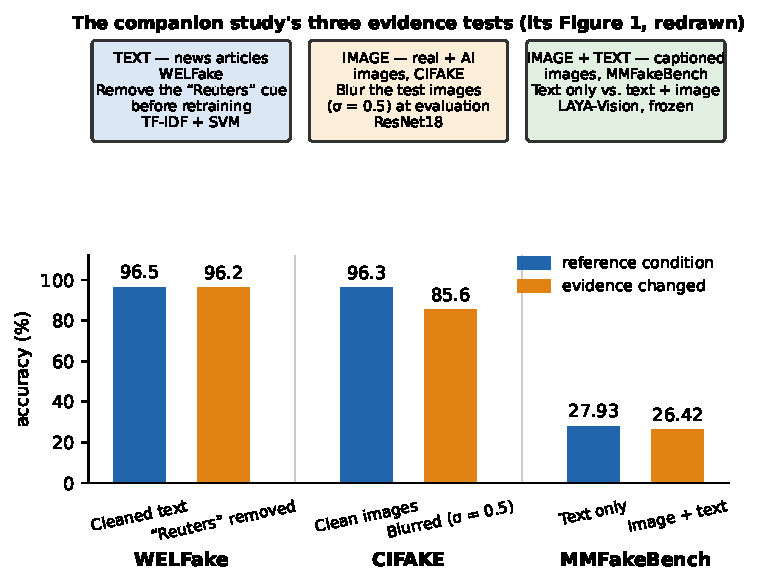
\includegraphics[width=\textwidth]{figures/fig_sard.pdf}
\caption{The companion study's three evidence tests and their accuracies. Top: the three tests as drawn in the companion study's opening figure (Seidenberg Annual Research Day (SARD), Pace University, 11 December 2026), redrawn. Bottom: accuracy in the reference condition and in the changed-evidence condition. On WELFake, a TF-IDF support vector machine scores 96.5\% on cleaned text and 96.2\% after the ``Reuters'' cue is removed; on CIFAKE, a fine-tuned ResNet18 scores 96.3\% on clean images and 85.6\% after Gaussian blur at evaluation; on MMFakeBench, frozen LAYA-Vision scores 27.93\% with text alone and 26.42\% with image and text. These are the companion study's results, measured with frozen models; this paper's own results are in Section~\ref{sec:experiments}.}
\label{fig:sard}
\end{figure}

Most current progress is dominated by large vision-language models (LVLMs) and agent frameworks. Contrastively pretrained encoders such as CLIP \citep{Radford2021LearningTransferable}, instruction-tuned assistants such as LLaVA and InstructBLIP \citep{Liu2023VisualInstruction, Dai2023InstructblipTowards}, and compact LVLMs \citep{Zhu2024LlavaphiEfficient} provide strong zero-shot image--text representations. Agent wrappers compose these models with tools and retrieval: HuggingGPT and ViperGPT turn multimodal inference into programmed tool use \citep{Shen2023HugginggptSolving, Surs2023VipergptVisual}; SNIFFER adds external evidence for explainable out-of-context detection \citep{Qi2024SnifferMultimodal}; MMD-Agent integrates reasoning and tools on MMFakeBench \citep{Liu2024MmfakebenchMixedsource}. Subsequent systems add evidence retrieval, type-aware reasoning, or test-time search; while promising, they frequently use validation, retrieval, or private re-split protocols that make their published figures difficult to compare directly. These systems often require frontier APIs, external retrieval, test-time search, or private re-splits, and operational cost is rarely disclosed.

Fine-tuned detectors offer a smaller alternative. Early multimodal fake-news systems learned shared representations or event-invariant features \citep{Khattar2019MvaeMultimodal, Wang2018EannEvent, Singhal2019SpotfakeMultimodal}; standard visual-language transformers such as LXMERT and VisualBERT remain common baselines \citep{Tan2019LxmertLearning, Li2019VisualbertSimple}. Parameter-efficient fine-tuning, especially LoRA and related low-rank recipes, makes small-data adaptation cheap \citep{Hu2021LoraLowrank, Kalajdzievski2023RankStabilization, Shuttleworth2024LoraVs}. Yet existing fine-tuned detectors often rely on larger external datasets, leave their split conventions unstated, or do not pre-register hyperparameters, which makes stability and transfer properties hard to audit.

Two further problems recur. First, evaluations leak. Dataset bias can inflate performance through annotation artifacts or metadata shortcuts \citep{Gururangan2018AnnotationArtifacts, Gebru2018DatasheetsDatasets}; leakage and reproducibility failures are widespread in machine-learning-based science \citep{Kapoor2023LeakageReproducibility, Pineau2020ImprovingReproducibility, Kapoor2024ReformsConsensusbased}. In our audit, a metadata-only rule reaches 0.9150 macro-F1 on the MMFakeBench tune split, a leakage ceiling that we report as a benchmark warning. Second, calibration is fragile: fitted temperatures are often treated as model properties even though calibration depends on the model--distribution pair \citep{Guo2017CalibrationModern, Naeini2015ObtainingWell, Ovadia2019CanYou, Minderer2021RevisitingCalibration}.

Typed-decision models are a much smaller alternative. Instead of generating free text, a typed-decision model reads a structured state plus a typed question and returns calibrated probabilities over a fixed option set in a single forward pass. LAYA-Vision, a 201M-parameter typed-decision vision-language model used in this study, follows this design. Our preceding diagnostic study found that the pretrained model does not perform multimodal misinformation detection zero-shot: it collapses onto a single class on MMFakeBench, a TF-IDF logistic baseline implemented with scikit-learn \citep{Pedregosa2011ScikitlearnMachine} roughly doubles its macro-F1, and a frozen-feature probe shows its representation carries signal that its decision head does not use.

This paper reports a pre-registered fine-tuning study of LAYA-Vision across three benchmarks whose definitions of falsity differ: MMFakeBench \citep{Liu2024MmfakebenchMixedsource}, NewsCLIPpings \citep{Luo2021NewsclippingsAutomatic}, and VERITE \citep{Papadopoulos2023VeriteRobust}. The contribution is primarily methodological: we do not introduce a new architecture or training algorithm. Instead, we show that a small typed-decision model, when embedded in a pre-registered, receipted protocol with explicit leakage and calibration checks, can yield one strong, one null, and one flat result across three benchmarks. We freeze a single protocol before evaluation: selection on tune only, the MMFakeBench test split scored exactly once, calibration fitted only on a reserved split, and all training runs receipted. The main grid compares full encoder-plus-head and LoRA arms under two objectives and three step budgets; a supplementary ablation tier runs after selection and never feeds it. Pre-registered hypotheses H1--H5 cover MMFakeBench gain, a NewsCLIPpings trained arm, VERITE transfer, per-class recall floors, and calibration.

The study yields three main results. First, on the directly comparable official MMFakeBench test protocol, a 201M model fine-tuned on 490 examples reaches 0.6020 macro-F1, with per-prediction inference cost around \$0.04 per 1,000 items and zero external dependencies. Second, the same recipe produces a null result on NewsCLIPpings (trained 0.5104 accuracy versus 0.5141 for this run's baseline) and near-flat transfer to VERITE (0.3506 versus 0.3467), showing that the gains are dataset-conditional. Third, methodological findings have independent value: a calibration temperature fitted on one distribution can harm held-out calibration, while a distribution-matched fit repairs it; a metadata leakage ceiling of 0.9150 exposes a benchmark shortcut; and the MMFakeBench literature is fragmented across at least six incompatible protocols. Throughout, we report negative results unsoftened and provide complete accounting of metered GPU cost, latency, artifact size, and deviations.

The fine-tuning results leave two questions open, and this paper pursues both in an integrated second part rather than a separate report. First, the diagnosis of Part I is that NewsCLIPpings and VERITE falsity is per-item and factual, a matter of what actually happened, where MMFakeBench falsity is stylistic and learnable from a few hundred examples. If that diagnosis is right, the natural remedy for the factual benchmarks is evidence supplied at inference time. Section~\ref{sec:evidencegate} registers and runs that test: a retrieval gate (EvidenceGate) that fetches external evidence for an item before judging it, an evidence-training stage that teaches the model to judge with evidence in context, and a four-arm track on VERITE. The section also reports, as part of the result, the situations the probe faced: its retrieval instrument failed silently and was repaired, its first repair was lost and redone, and its headline stage result did not survive an audit of its own scorer. Second, the binary screen beside the choice question ranked near chance in Part I (AUC 0.529 on NewsCLIPpings). Section~\ref{sec:noul} tests whether the screen's wording is the cause, screening six frozen wordings per dataset on the base model and following the deployments through a small training test and one frozen reporting evaluation. Section~\ref{sec:threats} collects the threats to validity of both parts. The probe's registrations, like Part I's hypotheses, were frozen before its results were scored.

Two contributions of the whole study are methodological, and they are named here so they can be cited as such. The first is an \textbf{abstention-accounting standard} for arbitrated verdicts: whenever a headline metric counts an abstention as an error, the accuracy including abstentions, the decided fraction, and the per-class headline recalls are co-primary, and no headline is quoted without them. Part II shows why the standard is needed: both of its headline-scale effects were movements in the decided fraction, in opposite directions. The second is the \textbf{warnings section} (Section~\ref{sec:threats}): a collected set of measured warnings for benchmark users, covering the 0.9150 metadata leakage ceiling, the calibration-transfer harm, the fragility of fitted operating points at small \(n\), and the abstention trap itself.

\section{Related Work}
\label{sec:related_work}
%%%%%%%%% RELATED WORK %%%%%%%%%%
We organize related work into three technical clusters: large vision-language models and agent frameworks, fine-tuned multimodal detectors and parameter-efficient fine-tuning, and calibration, dataset bias, and benchmark protocol fragmentation.

\subsection{Large Vision-Language Models and Agent Frameworks}
Large-scale contrastive pretraining, instruction tuning, and efficient multimodal assistants have reshaped image--text classification. CLIP \citep{Radford2021LearningTransferable}, LLaVA \citep{Liu2023VisualInstruction}, InstructBLIP \citep{Dai2023InstructblipTowards}, and compact LVLMs such as LLaVA-Phi \citep{Zhu2024LlavaphiEfficient} provide powerful zero-shot or instruction-following backbones. On multimodal misinformation tasks, however, the most visible recent systems wrap these models in agent loops. HuggingGPT and ViperGPT compose external tools through generated programs \citep{Shen2023HugginggptSolving, Surs2023VipergptVisual}; SNIFFER performs two-stage instruction tuning and retrieves external knowledge for out-of-context explanations \citep{Qi2024SnifferMultimodal}; MMD-Agent integrates reasoning, action, and tool use for MMFakeBench \citep{Liu2024MmfakebenchMixedsource}. Benchmarks such as MFC-Bench and LVLM studies further document sensitivity to manipulated content and evaluation design \citep{Wang2024MfcbenchBenchmarking, Tahmasebi2024MultimodalMisinformation}. These systems commonly assume frontier APIs, external retrieval, or test-time search, and their results are often reported under different split and metric regimes. Older cross-modality encoders such as LXMERT and VisualBERT remain standard comparison points on NewsCLIPpings-style data \citep{Tan2019LxmertLearning, Li2019VisualbertSimple}. Our work is not an agent system: it is a single forward-pass typed-decision classifier with zero external dependencies, and its reported costs and split labels are explicit.

\subsection{Fine-Tuned Multimodal Detectors and Parameter-Efficient Fine-Tuning}
Fine-tuned multimodal detectors predate large LVLM agents. Event-adversarial networks remove event-specific features \citep{Wang2018EannEvent}, multimodal variational autoencoders learn shared representations \citep{Khattar2019MvaeMultimodal}, and early frameworks such as SpotFake fuse BERT and VGG features without auxiliary subtasks \citep{Singhal2019SpotfakeMultimodal}. Cross-modality transformers such as LXMERT and VisualBERT provide strong baselines \citep{Tan2019LxmertLearning, Li2019VisualbertSimple}. Parameter-efficient fine-tuning (PEFT) makes adaptation cheaper. LoRA injects low-rank updates into frozen weights \citep{Hu2021LoraLowrank}; later work improves rank allocation \citep{Zhang2023AdaloraAdaptive}, analyzes learning-rate asymmetries \citep{Hayou2024LoraEfficient}, compares LoRA with full fine-tuning through spectral structure \citep{Shuttleworth2024LoraVs}, and stabilizes rank scaling \citep{Kalajdzievski2023RankStabilization}. Vector-based random-matrix adaptation further reduces parameter counts \citep{Kopiczko2023VeraVectorbased}. For vision-language models, adapter-style and training-free cache approaches improve few-shot transfer \citep{Gao2021ClipadapterBetter, Zhang2022TipadapterTrainingfree}, and unified views of visual PEFT compare these recipes \citep{Yu2022TowardsUnified}. In our study, a standard LoRA arm and a full encoder-plus-head arm are pre-registered, selected only on a tune split, and evaluated across datasets. We also report rank-stability hazards under this recipe rather than selecting the best post hoc.

\subsection{Calibration, Dataset Bias, and Benchmark Protocol Fragmentation}
Modern neural networks can be miscalibrated, and temperature scaling is a standard mitigation \citep{Guo2017CalibrationModern, Naeini2015ObtainingWell}. However, calibration is not a fixed model property: it degrades under dataset shift \citep{Ovadia2019CanYou, Minderer2021RevisitingCalibration}, which motivates distribution-aware and non-parametric calibration methods \citep{Kull2019BeyondTemperature, Kumar2019VerifiedUncertainty, Vaicenavicius2019EvaluatingModel, Gupta2020CalibrationNeural, Nixon2019MeasuringCalibration, Barber2019ConformalPrediction, Gibbs2021AdaptiveConformal}. Our experiments provide a concrete instance of this distribution dependence: a temperature fitted on one split raises held-out ECE, while a split-half fit repairs it. Dataset bias and leakage are equally important. Annotation artifacts can make label prediction possible from partial inputs \citep{Gururangan2018AnnotationArtifacts}; leakage taxonomies and reproducibility programs show how such shortcuts lead to overoptimistic conclusions \citep{Kapoor2023LeakageReproducibility, Pineau2020ImprovingReproducibility, Kapoor2024ReformsConsensusbased}. Dataset documentation standards such as datasheets support the disclosure of metadata and intended use \citep{Gebru2018DatasheetsDatasets}. In this study we report a 0.9150 metadata leakage ceiling on MMFakeBench and formally refuse to feed source metadata to the model. Finally, because benchmark scores are often averaged or transferred across tasks, we separate datasets and transfer results rather than aggregating them; this echoes the separation of average accuracy from transfer in continual-learning evaluation \citep{Lopezpaz2017GradientEpisodic}.
%%%%%%%%% RELATED WORK %%%%%%%%%%

\section{Methodology}
\label{sec:method}
%%%%%%%%% METHOD %%%%%%%%%%
\subsection{Typed-Decision Formulation and Dataset Packs}
Let an image--text pair be \(x=(t,v)\), where \(t\) is the context text and \(v\) is the image. Let \(\mathcal{Y}\) be the fixed label set of a dataset pack. A typed-decision model \(M_\theta\) maps the pair and a dataset-specific typed question \(q\) to a distribution over \(\mathcal{Y}\):
\[
p(y\mid x,q;\theta)=M_\theta(x,q),
\qquad
\hat{y}=\mathop{\mathrm{arg\,max}}_{y\in\mathcal{Y}}\,p(y\mid x,q;\theta).
\]
Every evaluation call returns two questions in one forward pass: a native choice question over the dataset's own classes, and a binary fake screen expressed as a \( \texttt{noul} \) probability question. The choice verdict is the headline; the screen is reported beside it, and disagreement between the two is labeled as uncertain.

Per-dataset packs fix the questions, label spaces, native metrics, and calibration behavior. Specifically, MMFakeBench uses four classes (original, textual veracity distortion, visual veracity distortion, mismatch) and macro-F1; NewsCLIPpings uses pristine versus falsified and accuracy; VERITE uses truthful, miscaptioned, and out-of-context and three-class accuracy. These metrics are never averaged across datasets.

Gold labels, item IDs, file paths, and source metadata are never model inputs. To measure the risk of shortcut learning, we define a metadata-only rule that reads only the two provenance fields \( \texttt{text\_source} \) and \( \texttt{image\_source} \), maps each observed source combination to the most frequent label, and predicts every item with that provenance as that label. This rule uses no image or text content. It reaches 0.9150 macro-F1 on the MMFakeBench tune split, and 0.9150 accuracy / 0.8510 macro-F1 on the official test split. We report this leakage ceiling as a benchmark warning rather than as a model result. This audit is deliberately narrow: it examines only explicit source metadata. It does not test for content-based source-identifying cues such as watermarks, text style, or image artifacts. The ceiling therefore demonstrates that a metadata-only shortcut exists; it does not quantify every possible shortcut signal in the benchmark.

\subsection{Model Architecture and Trainable Arms}
LAYA-Vision is a 201M-parameter typed-decision vision-language model with a language encoder and a two-layer decision head. The checkpoint used is \( \texttt{thaitea/laya-vision} \) at pinned revision \( \texttt{f2fe3c12cb6d04c59d8a190250bf3fb40fc828dc} \). The model does not generate free text; it returns probabilities over a fixed option set in a single forward pass. The checkpoint is used exactly as released, and fine-tuning does not modify the architecture. Figure~\ref{fig:arch} shows the computation.

\begin{figure}[t]
\centering
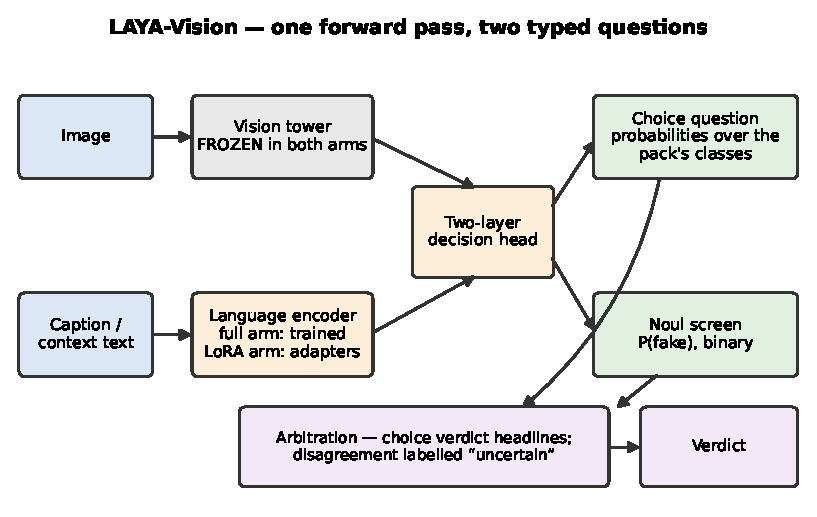
\includegraphics[width=\textwidth]{figures/fig_arch.pdf}
\caption{LAYA-Vision as used in this study. An image--text pair enters one forward pass: the vision tower is frozen in both training arms; the language encoder and the two-layer decision head are trained, directly in the full arm and through low-rank adapters in the LoRA arm; and the head answers two typed questions, a native choice question over the dataset pack's classes and a binary fake screen. The choice verdict headlines; disagreement between the two answers is labelled uncertain.}
\label{fig:arch}
\end{figure}

We compare two trainable arms. The full arm trains the language encoder and decision head, with 114,728,323 of 201,161,347 parameters trainable. The vision tower is frozen in both arms due to a library limitation; following the binding labelling rule, this arm is always described as encoder-plus-head fine-tuning, never full-model fine-tuning. The LoRA arm follows \citet{Hu2021LoraLowrank} with rank \(r=16\), scaling factor \( \alpha=32\), dropout \(0.05\), and targets the query, value, key, output, gate, up, and down projections. Its learning rate is \( \texttt{lr\_lora}=0.001\), and it is always reported as such. Rank-scaling issues are relevant because higher ranks are explored in the supplementary tier \citep{Kalajdzievski2023RankStabilization}.

\subsection{Fine-Tuning Objectives and Frozen Protocol}
The main grid uses the training library's two built-in objectives. For every dataset pack, the training library produces a fixed soft target from the pack definition. We use the pinned library implementation as the authoritative specification: we do not infer the target construction from external mathematics and do not replace it with an ad-hoc smoothing rule. Let \(p_\theta(c\mid x,q)\) be the model probability for class \(c\), and let \(\tilde{p}_{\mathrm{soft}}(c\mid x,q)\) be the library-defined soft target for the active dataset pack. The \( \texttt{soft\_ce} \) objective is
\[
\mathcal{L}_{\mathrm{soft\_ce}}(\theta)
=
-\frac{1}{n}
\sum_{i=1}^{n}
\sum_{c\in\mathcal{Y}}
\tilde{p}_{\mathrm{soft}}(c\mid x_i,q_i)
\log p_\theta(c\mid x_i,q_i),
\]
where the soft targets are fixed by the dataset pack and are not learned from any evaluation split. The \( \texttt{rlcd} \) objective is the library's built-in \( \texttt{rlcd} \) term and is likewise defined by the pinned code. Because the identity of the library's \( \texttt{rlcd} \) objective relative to published RLCD methods is unresolved, we deliberately refrain from writing an external mathematical definition for it and do not claim that it corresponds to a published RLCD loss. Every soft-ce-versus-rlcd claim is scoped as ``within this library's two objectives, under this recipe,'' never as a claim about RLCD in general.

The MMFakeBench development partition is frozen as 490 train items (980 records, with each item in both question forms), 105 tune items (210 records), and 105 calibration items (210 records). This partition is carved from the official 1,000-item MMFakeBench validation split; the official 10,000-item test split is not used for selection, calibration, or any adaptation step. Selection uses only the tune split. The MMFakeBench test split is scored exactly once, by the frozen winner, after selection. Calibration is fitted only on the reserved calibration split after selection. Gold labels, item IDs, file paths, and source metadata are never model inputs.

\subsection{Hypotheses and Evaluation Metrics}
We pre-register five binary hypotheses before evaluation.
\begin{itemize}
    \item \textbf{H1 (MMFakeBench gain):} the winning configuration improves test macro-F1 over the pretrained baseline by at least \(+0.03\), with paired-resampling 95\% CI lower bound greater than zero and no per-class recall drop larger than 5 percentage points.
    \item \textbf{H2 (NewsCLIPpings trained arm, as re-aimed by amendment (c)):} validation accuracy falls in the \(0.55\)--\(0.65\) band and beats the zero-shot figure by at least \(+6.24\) points. The 6.24-point bar is the October frozen-representation probe's measured gain over zero-shot on NewsCLIPpings (\(+6.24\) points, interval \([4.76, 7.70]\)), adopted at the re-aim as the improvement the fine-tuned arm had to match.
    \item \textbf{H3 (VERITE transfer):} the MMFakeBench winner, transferred without VERITE training, reaches accuracy in the \(0.38\)--\(0.48\) band.
    \item \textbf{H4 (recall floor):} the minimum per-class tune recall of the winner is at least \(0.25\).
    \item \textbf{H5 (calibration):} calibration fitted on the reserved calibration split brings tune expected calibration error under \(0.15\), with accuracy unchanged.
\end{itemize}

For expected calibration error, we use the standard binned estimator:
\[
\mathrm{ECE}
=
\sum_{m=1}^{M}
\frac{|B_m|}{n}
\left|
\mathrm{acc}(B_m)
-
\mathrm{conf}(B_m)
\right|,
\]
where \(B_m\) is the \(m\)-th confidence bin. Negative log-likelihood is computed as
\[
\mathrm{NLL}
=
-\frac{1}{n}
\sum_{i=1}^n
\log p(y_i\mid x_i,q;\theta).
\]
Paired resampling confidence intervals use 2,000 resamples, and differences between systems are stated in percentage points rather than as bare percent changes.

\section{Experiments}
\label{sec:experiments}
%%%%%%%%% EXPERIMENTS %%%%%%%%%%
\subsection{Experimental Setup and Cost Ledger}
Training uses seed 20261122, maximum sequence length 1024, batch size 8, and bf16 precision. The full arm uses \( \texttt{lr\_encoder}=1\times10^{-5} \) and \( \texttt{lr\_head}=1\times10^{-3} \). The LoRA arm uses \( \texttt{lr\_lora}=0.001 \). For MMFakeBench, the development partition is carved from the official 1,000-item validation split as stated in Section~\ref{sec:method}; the full validation split is scored as an internal check, and the official 10,000-item test split is scored only once at the end. The NewsCLIPpings trained arm is carved from its official train split only: 2,501 items over 2,120 unique images, divided into 2,001 train items, 250 tune items, and 250 calibration items. This carve is a registration-driven subset, not a sample from arbitrary data, and its size follows from the run machine's storage budget under the saved training-subset exception: evaluation must stream the 91 GB VisualNews archive, whereas the carve saves exactly the official train-split items needed for the arm. Selection on NewsCLIPpings uses the native question form only because the two question forms have flipped label indices; evaluation uses streamed official validation rows.

Table~\ref{tab:cost} reports the Part I cost ledger. It excludes human engineering time, data acquisition, and environmental externalities, which are not metered by the run machine. Part I lived on one secure RTX 4090 pod for about 7.6 hours at \$0.90 per hour all-in; total pod spend was about \$6.83 (start balance \$9.7725, a mid-run credit of about \$10.05, final balance \$12.9967; the credit term is a bracketed estimate, so the spend carries about \$0.10 of uncertainty). Metered training time across all 29 trainings totals \$2.14; pre-run sunk costs were \$0.17 (rehearsal) and \$0.72 (pre-grid burn). Inference is measured at 0.16 seconds per item on the run machine, corresponding to about \$0.04 per 1,000 predictions. Notebook-only execution on the run machine's Jupyter kernel is recorded as a deviation. The ledger in Table~\ref{tab:cost} covers Part I only; the probe of Sections~\ref{sec:evidencegate} and~\ref{sec:noul} ran in separately metered sessions, and its closing phase cost \$3.3391 against a \$5 phase hard stop. The probe's remaining metered spend is also on the record: about \$3.05 on its first pod, \$1.20 of idle burn on a replacement pod that was never reachable, about \$0.14 on the driver-wedged pod, and about \$0.50 of retrieval, repair, and assembly calls. Figure~\ref{fig:pipeline} summarises the frozen pipeline end to end.

\begin{figure}[t]
\centering
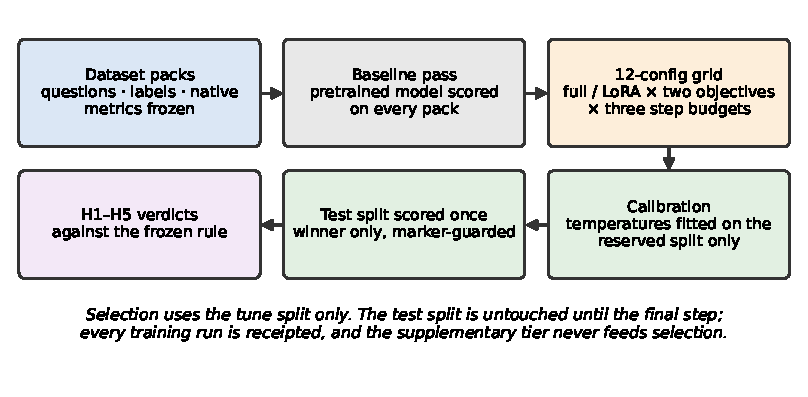
\includegraphics[width=\textwidth]{figures/fig_pipeline.pdf}
\caption{The frozen experiment pipeline. Dataset packs fix the questions, label spaces, and native metrics before any scoring; selection uses the tune split only; calibration is fitted on the reserved split after selection; and the official test split is scored exactly once, by the frozen winner.}
\label{fig:pipeline}
\end{figure}

\begin{table}[t]
\centering
\small
\caption{Measured cost and operational characteristics (Part I, the fine-tuning programme).}
\label{tab:cost}
\begin{tabular}{ll}
\toprule
Item & Value \\
\midrule
Total pod spend & \(\approx \$6.83\) \\
Metered training time, 29 trainings & \(\$2.14\) \\
Rehearsal cost & \(\$0.17\) \\
Pre-grid burn & \(\$0.72\) \\
Pod rate & \(\$0.90\)/hour \\
Pod duration & \(\approx 7.6\) hours \\
Inference latency & 0.16 s/item \\
Inference cost & \(\approx \$0.04\) per 1,000 predictions \\
Artifact size & \(\approx 805\) MB \\
\bottomrule
\end{tabular}
\end{table}

\subsection{MMFakeBench Grid Selection and Headline Test Result}
Table~\ref{tab:grid} ranks all 12 pre-registered grid configurations by tune macro-F1. The frozen winner is \( \texttt{full\_soft\_ce\_735} \), with tune macro-F1 0.7389 and tune accuracy 0.7429. Within this library's two objectives and under this recipe, soft-ce beats rlcd in all six matched pairs. Two failure modes are recorded: the full-rlcd training loss falls to approximately 0.00, and \( \texttt{lora\_rlcd\_735} \) collapses onto the original class with tune macro-F1 0.1946. Figure~\ref{fig:grid} presents the same selection as a heatmap.

\begin{table}[t]
\centering
\small
\caption{MMFakeBench grid selection on the tune split.}
\label{tab:grid}
\begin{tabular}{lcc}
\toprule
Configuration & Tune macro-F1 & Tune accuracy \\
\midrule
full\_soft\_ce\_735 & 0.7389 & 0.7429 \\
lora\_soft\_ce\_735 & 0.7187 & 0.7048 \\
full\_soft\_ce\_490 & 0.6598 & 0.6667 \\
lora\_soft\_ce\_245 & 0.6282 & 0.6571 \\
full\_rlcd\_735 & 0.6061 & 0.6190 \\
full\_soft\_ce\_245 & 0.5954 & 0.6000 \\
full\_rlcd\_490 & 0.5880 & 0.6000 \\
lora\_soft\_ce\_490 & 0.5726 & 0.5810 \\
full\_rlcd\_245 & 0.5667 & 0.5619 \\
lora\_rlcd\_245 & 0.4597 & 0.5905 \\
lora\_rlcd\_490 & 0.4505 & 0.6095 \\
lora\_rlcd\_735 & 0.1946 & 0.3333 \\
\bottomrule
\end{tabular}
\end{table}

\begin{figure}[t]
\centering
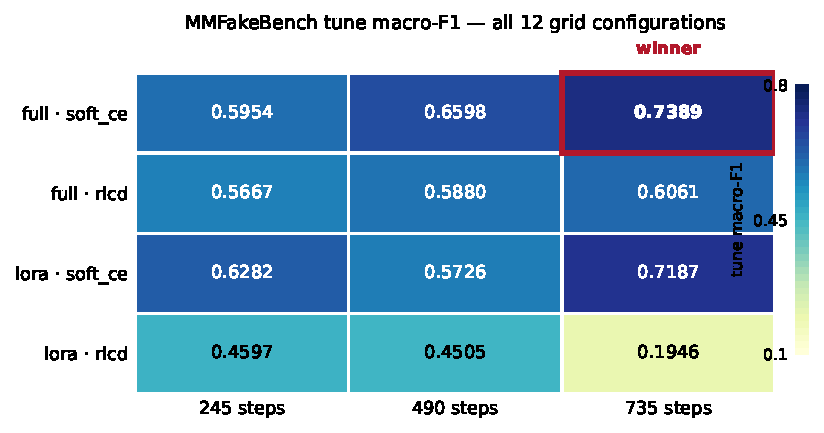
\includegraphics[width=\textwidth]{figures/fig_grid.pdf}
\caption{The MMFakeBench grid of Table~\ref{tab:grid} as a heatmap (tune macro-F1, \(n = 105\) tune items). The frozen winner, full encoder-plus-head with soft-ce at 735 steps (0.7389), is outlined.}
\label{fig:grid}
\end{figure}

The winner's per-class tune recalls are 0.656 for original, 0.969 for textual veracity distortion, 0.700 for visual veracity distortion, and 0.613 for mismatch. On the full validation split, the winner reaches accuracy 0.7690, while the pretrained baseline under the same frozen wording reaches accuracy 0.293 and macro-F1 0.2079. Table~\ref{tab:mmfake} summarizes the headline test result. The official MMFakeBench test split is scored exactly once, on 9,999 paired rows with the single undecodable item excluded symmetrically from both arms. The winner reaches macro-F1 0.6020 versus baseline 0.2037. Paired resampling gives \(\Delta=+0.3983\), 95\% CI \([+0.3853, +0.4108]\). Every per-class recall improves. An error analysis of the winner's stored test predictions (Section~\ref{sec:evidencegate} returns to the pattern) shows where the remaining errors sit: of 3,870 errors, the original-versus-mismatch boundary carries 2,375 (mismatch called original 1,424; original called mismatch 951), while textual distortion is the strong class (recall 0.8343). Accuracy by text source ranges from 0.972 (Gossipcop) to 0.258 (DGM4).

The validation-to-test gap for the winner is large: 0.7690 validation accuracy versus 0.6130 test accuracy. This is not a general test-time protocol failure, because the pretrained baseline is nearly flat across the same two splits in macro-F1 (0.2079 validation versus 0.2037 test). Instead, the gap is consistent with selection on a small 105-item tune split and specialization to validation-style examples, while the official test contains 10,000 image--text pairs and a broader source/label composition. The per-class test recalls show that the largest remaining errors are on visual veracity distortion (0.512) and mismatch (0.422). By design, we do not use the test split to adapt the model or to select a different configuration after this single scoring. Figure~\ref{fig:headline} collects the before-and-after headline result for each of the three datasets on a common scale.

\begin{table}[t]
\centering
\small
\caption{Official MMFakeBench test result and per-class recalls.}
\label{tab:mmfake}
\begin{tabular}{lcc}
\toprule
Metric & Baseline & Winner \\
\midrule
Validation accuracy & 0.293 & 0.7690 \\
Validation macro-F1 & 0.2079 & n/r \\
Test macro-F1 & 0.2037 & 0.6020 \\
Test accuracy & n/r & 0.6130 \\
\midrule
Test recall: original & 0.213 & 0.617 \\
Test recall: textual & 0.524 & 0.834 \\
Test recall: visual & 0.026 & 0.512 \\
Test recall: mismatch & 0.135 & 0.422 \\
\bottomrule
\end{tabular}
\end{table}

\begin{figure}[t]
\centering
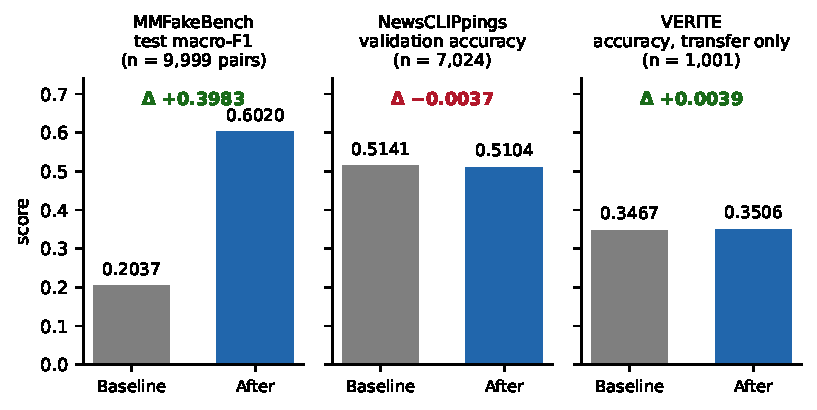
\includegraphics[width=\textwidth]{figures/fig_headline.pdf}
\caption{Before-and-after headline results, one panel per dataset, each on its native metric. Left: MMFakeBench test macro-F1, baseline 0.2037 to winner 0.6020. Centre: NewsCLIPpings validation accuracy, baseline 0.5141 to trained 0.5104, a null result. Right: VERITE accuracy under transfer only, baseline 0.3467 to 0.3506, near-flat. The three metrics are never averaged across datasets.}
\label{fig:headline}
\end{figure}

\subsection{NewsCLIPpings Trained Arm and Streamed Evaluation}
Table~\ref{tab:ncp} reports the NewsCLIPpings arm. The training carve uses only official train-split rows, so no validation or test rows enter training. The pretrained baseline scores 7,024 out of 7,024 streamed validation rows with accuracy 0.5141 and predicts falsified for 93\% of rows. The trained winner scores the same rows with accuracy 0.5104: a null result against this run's own baseline. Macro-F1, which is not the pack's native metric, moves the other way (0.4036 for the baseline to 0.4436 for the trained arm) on the rebalancing toward pristine; the registered verdict reads on accuracy, and on accuracy nothing moves. Its pristine recall is 0.164, falsified recall is 0.857, binary-screen AUC is 0.529, and mean confidence is approximately 0.500. The trained model still predicts falsified for 84.6\% of pairs.

Although the trained arm makes fewer falsified calls than the baseline, it barely moves accuracy. With mean confidence near \(0.500\) and binary-screen AUC 0.529, the model does not learn a useful confidence-separated boundary and instead remains dominated by the falsified class. The pristine recall improves only from 0.084 to 0.164.

\begin{table}[t]
\centering
\small
\caption{NewsCLIPpings streamed validation results.}
\label{tab:ncp}
\begin{tabular}{lcc}
\toprule
Metric & Baseline & Trained winner \\
\midrule
Accuracy & 0.5141 & 0.5104 \\
Macro-F1 & 0.4036 & 0.4436 \\
Pristine recall & 0.084 & 0.164 \\
Falsified recall & 0.944 & 0.857 \\
Binary-screen AUC & 0.549 & 0.529 \\
\bottomrule
\end{tabular}
\end{table}

H2 is \textbf{NOT MET} under the re-aimed criterion. The trained winner's accuracy is only \(+0.2\) percentage points over October's 0.5083 and \(-0.4\) percentage points against this run's own baseline; at \(n=250\), the tune interval is roughly \([0.446, 0.570]\), so this margin is not a proven edge.\footnote{This run's baselines were measured with the frozen pack question wording; October's used different wording, and the baseline moved on identical rows (MMFakeBench validation accuracy \(0.320\rightarrow0.293\); NewsCLIPpings \(0.5083\rightarrow0.5141\); VERITE \(0.3566\rightarrow0.3467\)). October measured \(\pm0.03\) phrasing swings. Comparisons use one wording consistently or carry this footnote.} The temperature gate is mechanical: fitted NewsCLIPpings temperatures \([3.857, 2.100, 3.053]\) give held-out ECE 0.0127 versus raw ECE 0.0120, so the published NewsCLIPpings pack ships \(T=1.0\).

\subsection{VERITE Transfer}
Table~\ref{tab:verite} reports transfer-only results on 1,001 local rows of the official 1,000-item dataset. Our local extraction contains one additional row, so we score all local rows without ad-hoc filtering. No VERITE training is performed. The MMFakeBench winner transfers to VERITE with accuracy 0.3506, essentially flat relative to the baseline 0.3467. Per-class recalls are 0.808 for truthful, 0.148 for miscaptioned, and 0.086 for out-of-context. H3 is \textbf{NOT MET}; fine-tuning specialized the model for MMFakeBench's style of falsity and bought essentially nothing on VERITE's.

The transferred model differs from the baseline on 543 of 1,001 labels yet nets only \(+0.4\) percentage points accuracy and slightly lower macro-F1 (0.2798 versus 0.2819). This indicates label churn rather than useful transfer: the model is confident on truthful items but fails to separate VERITE's miscaptioned and out-of-context classes.

\begin{table}[t]
\centering
\small
\caption{VERITE transfer-only results.}
\label{tab:verite}
\begin{tabular}{lcc}
\toprule
Metric & Baseline & MMFakeBench winner transferred \\
\midrule
Accuracy & 0.3467 & 0.3506 \\
Macro-F1 & 0.2819 & 0.2798 \\
Truthful recall & 0.429 & 0.808 \\
Miscaptioned recall & 0.009 & 0.148 \\
Out-of-context recall & 0.612 & 0.086 \\
\bottomrule
\end{tabular}
\end{table}

\subsection{Calibration Analysis and H5}
Table~\ref{tab:calib} reports the registered calibration measurements, and Figure~\ref{fig:cal1} draws them together. On the reserved calibration split, fitted scaling reduces ECE from 0.2664 to 0.0865 and NLL from 2.64 to 0.61; on the tune split the same temperature moves ECE from 0.1941 to 0.0778 with tune accuracy unchanged at 0.7857; H5 is \textbf{MET as registered}. However, when the fitted temperature \(T=8.4214\) is applied to the held-out MMFakeBench validation split, raw ECE 0.1056 worsens to 0.3955. A split-half fit on the same validation data yields \(T\approx1.65\), and held-out ECE improves from 0.0994 to 0.021. A full-validation fit gives \(T\approx1.6\).

\begin{table}[t]
\centering
\small
\caption{Calibration measurements under distribution shift.}
\label{tab:calib}
\begin{tabular}{lcc}
\toprule
Setting & Raw ECE & Fitted ECE \\
\midrule
Registered calibration split & 0.2664 & 0.0865 \\
Tune split, same \(T\) & 0.1941 & 0.0778 \\
Held-out validation, using split-fitted \(T=8.4214\) & 0.1056 & 0.3955 \\
Split-half validation, using half-fitted \(T\approx1.65\) & 0.0994 & 0.021 \\
\bottomrule
\end{tabular}
\end{table}

\begin{figure}[t]
\centering
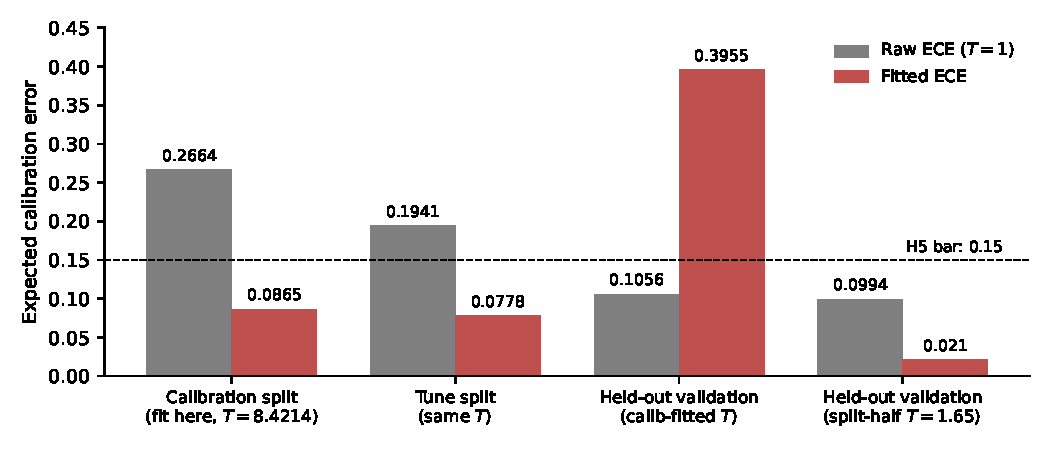
\includegraphics[width=\textwidth]{figures/fig_cal1.pdf}
\caption{The CAL-1 calibration picture. A temperature fitted on the calibration split (choice \(T=8.4214\); the score and screen temperatures stayed at 1.0) improves ECE where it was fitted and on the tune split, then severely harms held-out validation calibration (0.1056 to 0.3955). A split-half fit on the held-out distribution itself (\(T=1.65\); a full-validation fit gives \(T=1.6\)) repairs it (0.0994 to 0.021). A same-distribution fit transfers; a training-distribution fit does not. Both published packs therefore ship at \(T=1.0\).}
\label{fig:cal1}
\end{figure}

The disposition is as executed: H5 stands as registered with this qualification, the published MMFakeBench pack ships \(T=1.0\), and \(T\approx1.6\) is documented only as a deployment-calibration alternative. This is a concrete instance that a temperature is a property of model-times-distribution, not a model constant \citep{Guo2017CalibrationModern, Ovadia2019CanYou, Minderer2021RevisitingCalibration}.

\subsection{Supplementary Ablations, Protocol Audit, and Competitive Position}
The supplementary ablation tier runs after selection and never feeds selection, calibration, or test-once scoring. A second seed of the winner recipe reaches 0.7320, so the winner is not a lucky-seed artifact at the tune level. Encoder learning-rate variants score 0.7178, 0.6871, 0.6438, and 0.6217. LoRA rank r8 reaches 0.7037 at 490 steps, while r32 collapses or diverges: 0.1168 at 490 steps and 0.2244 at 735 steps with training loss rising from 0.762 to 1.070. At this data scale, higher LoRA rank is a stability hazard under the standard recipe. Head-only fine-tuning scores at most 0.4899 and is never described as a linear probe. The data-size curve collapses at 122 training items \((0.1168)\), improves to 0.3670 at 245 items, and reaches 0.6598 at 490 items, indicating a minimum-data cliff. Figure~\ref{fig:ablations} plots the data-size curve and the LoRA rank ladder.

\begin{figure}[t]
\centering
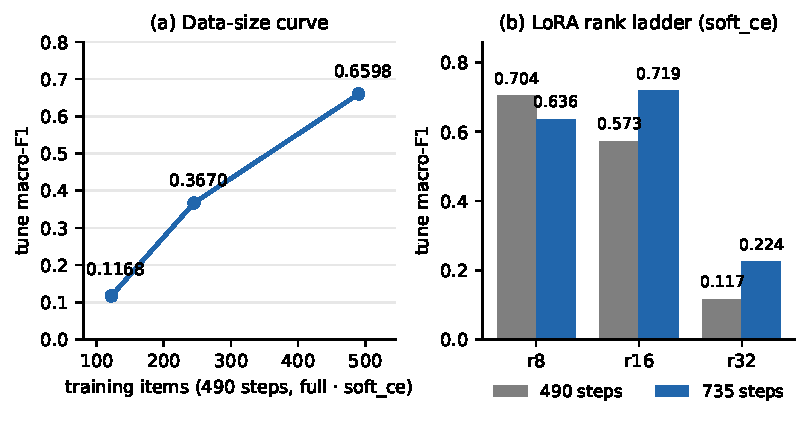
\includegraphics[width=\textwidth]{figures/fig_ablations.pdf}
\caption{Supplementary-tier behaviour on the MMFakeBench tune split. (a) The data-size curve at 490 steps: performance collapses at 122 training items (0.1168), recovers at 245 items (0.3670), and reaches 0.6598 at 490 items. (b) The LoRA rank ladder under soft-ce: rank 8 and rank 16 remain trainable at both step budgets, while rank 32 collapses. The rank-16 column is the main grid's LoRA arm.}
\label{fig:ablations}
\end{figure}

\begin{figure}[t]
\centering
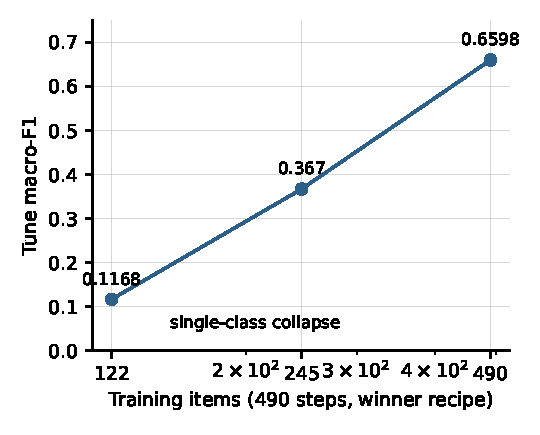
\includegraphics[width=0.55\textwidth]{figures/fig_datasize.pdf}
\caption{The data-size curve on its own (supplementary tier, winner recipe at a fixed 490 steps). At 122 training items the model collapses to a single class (tune macro-F1 0.1168); 245 items give 0.3670 and 490 items give 0.6598. The 0.1168 value is shared, to full precision, with the rank-32 supplementary run at 490 steps: both runs collapse to the same single-class prediction pattern on the same tune split, so the identity is a shared collapse value, not a copying error.}
\label{fig:datasize}
\end{figure}

We did not retrain standard vision-language baselines such as CLIP, VisualBERT, or LXMERT under the frozen 490-example protocol. This is a pre-registered single-model audit: adding multiple model families would produce a benchmark sweep rather than the receipted protocol study we froze. A benchmark sweep would also need to choose one of several incompatible protocols; since protocol fragmentation is one of the paper's findings, mixing new retrained baselines into only one of those protocols would not resolve the fragmentation and could be misleading. For external systems we therefore use published Protocol A results and label every protocol rather than creating new mixed comparisons.

Table~\ref{tab:protocol} separates Protocol A official-test results from non-comparable regimes. On Protocol A, LAYA-Vision trails only the frontier-model agent system and leads every fine-tuned system whose official-test split is verified. One further system, DeceptionDecoded, reports 58.66 under a Protocol A claim whose split we could not verify; it is tabled below the line with the non-comparable regimes, and no claim in this paper rests on the comparison. Other published numbers use validation, binary, retrieval, or private re-split protocols and are not directly comparable.

\begin{table}[t]
\centering
\small
\caption{Protocol-labelled MMFakeBench comparison.}
\label{tab:protocol}
\begin{tabular}{lcc}
\toprule
System & Protocol & Macro-F1 \\
\midrule
GPT-4V Standard & A: official test & 48.8 \\
GPT-4V + MMD-Agent & A: official test & 61.5 \\
LLaVA-1.6-34B Standard & A: official test & 25.7 \\
SCPO & A: official test, Top-1 extraction & 57.3 \\
LAYA-Vision (this study) & A: official test & 60.20 \\
\midrule
\multicolumn{3}{l}{\textit{Not Protocol A: not directly comparable}} \\
DeceptionDecoded & A claimed; split unverified & 58.66 \\
MERIT/MIRAGE & binary, validation, retrieval & 81.65 \\
T2Agent & validation, test-time search & 75.9 \\
MM-VeriAgent & private re-split & 71.5 \\
AgentM3D & validation & 62.6 \\
LRQ-FACT & validation & 71.6 \\
\bottomrule
\end{tabular}
\end{table}

Cost estimates for frontier systems are marked as estimates, not measurements. Scoring the 10,000-item test once via a GPT-4V-class API is estimated at about \$155, and an agent framework at roughly \$450--750. These are about 1,000 times the per-item cost of the LAYA forward pass.

\section{EvidenceGate: Retrieved Evidence at Inference and in Training}
\label{sec:evidencegate}
%%%%%%%%% EVIDENCEGATE %%%%%%%%%%
\subsection{Design and Registration}
EvidenceGate wraps the Part I model in a state machine. An item enters at Intake, is Routed (by dataset pack, and by an uncertainty trigger for the per-item route), goes to PairOnly or Retrieve, is Judged by LAYA-Vision with the evidence block in its context when retrieved, and passes through Arbitrate, the same choice-and-screen arbitration as Part I, to Done. Detached, the gate is byte-identical to the v1 pipeline; that was verified, not assumed. Retrieval ran in two variants: variant A built its search queries deterministically from extracted entities (an NLP-only pipeline), and variant B sent the same extracted spans to a small language-model harness, which returned a one-line claim and its own queries. The arms are P0 (pair-only), P1A (variant A pool, fact-check domains excluded, date rule enforced), P2A (the same variant A pool, fact-check domains included), and P1B (variant B pool, fact-check excluded and date-enforced). The probe set is 300 NewsCLIPpings validation items, stratified by gold class crossed with source stratum under seed 20261122 (152 pristine, 148 falsified). All evaluation items, thresholds, and success criteria for the probe were registered before the runs that used them.

\subsection{The Retrieval Collapse and Its Repair}
The first retrieval pass ran up to about 23 query streams at once. That tripped the search backend's unusual-traffic suspension, and with the fallback engine blocked by the network egress proxy, the search layer returned empty result lists silently. Counted from the snapshot files' pool sizes, empty (item, variant) pools were: probe 481 of 600, VERITE 375 of 400, Stage B carve 630 of 700, pilot 21 of 52. Those snapshots were failed retrievals, not retrieval results, and no judging was ever scored on them for the evidence arms.

The repair ran serially: one query at a time, one second apart, a circuit breaker that paused for 240 seconds after ten consecutive empty returns, frozen query lists unchanged. The first repair attempt reached 400 of 481 probe pairs but kept its output in memory and lost it when the session ended; the script was then patched to checkpoint every pair to disk and to resume idempotently, and the repairs completed. Final states: probe 597 of 600 pairs non-empty (three pairs marked retrieval-failed; only one of them loses its headline pool), VERITE 349 of 400, Stage B carve 694 of 700. After assembly, with verdict-content, fact-check-claim, and same-source exclusions applied, headline coverage was 193 of 300 probe items (64.3 percent, above the registered 60 percent claim bar) and 89 of 200 VERITE held-out items (44.5 percent). The VERITE exclusions bit hard there (508 verdict-content and 377 fact-check-claim passages removed), which is itself part of the VERITE evidence result: items that originate from fact-check articles shed most of their retrievable context by design.

\subsection{Reproducibility Audit}
At probe end, the 30 pilot items were re-retrieved fresh, serially, with the same query lists, and their passage-URL sets compared against the frozen pools: 60 (item, variant) pairs, mean Jaccard 0.2161, median 0.1111. Live retrieval is not reproducible at a one-day lag; result sets drift with engine availability and ranking churn. That audit is the quantitative justification for the frozen snapshot design: every Part II number is computed against the hashed snapshots, and any replication must start from them, not from a fresh search. The audit's base is the 30 pilot items only, and the claim keeps that scope.

\subsection{Pilot}
Thirty items, the v1 NewsCLIPpings winner checkpoint, no verdict registered at this size. Pair-only headline accuracy 0.3667; evidence (P1A) 0.4000, paired delta \(+0.0333\) with interval \([-0.0667, +0.1667]\); P1B 0.4333. The pair-only labels agreed with the frozen v1 comparator on 29 of 30 items, which verified that the pod pipeline reproduced the v1 winner's behaviour before any larger run depended on it. The gate's own modes read: always-on evidence 0.4000, triggered routing 0.3333 with five flips blocked to uncertain, and a trigger fire rate of 1.0. The trigger fired on every pilot item, which is a finding about the trigger threshold against this model's confidence distribution, not about the gate's plumbing.

\subsection{Stage A: Evidence at the Frozen Model}
The v1 NewsCLIPpings winner judged the 300 probe items pair-only and with evidence, scored at the registered screen threshold of 0.5. All figures are the scorer audit's recomputation (Section~\ref{sec:scorer}).

\begin{table}[t]
\centering
\small
\caption{Stage A on the 300 probe items (frozen v1 NewsCLIPpings winner).}
\label{tab:stagea}
\begin{tabular}{lccc}
\toprule
Arm & Headline acc & Acc incl.\ uncertain & Uncertain \\
\midrule
P0 pair-only & 0.4300 & 0.5133 & 44 \\
P1A evidence & 0.4500 & 0.5300 & 56 \\
P2A evidence & 0.4500 & 0.5300 & 56 \\
P1B evidence & 0.3800 & 0.5067 & 80 \\
\bottomrule
\end{tabular}
\end{table}

Paired delta, P1A against P0: \(+0.0200\), interval \([-0.0267, +0.0667]\), under headline accounting; under the including-uncertain accounting the gap is 0.5300 against 0.5133. At fixed coverage the evidence arm is modestly ahead at every level (Figure~\ref{fig:coverage}). The strata cut the other way: items with no evidence score 0.4953 headline, items with binding evidence 0.4795, and items with corroboration only 0.3917, with falsified accuracy falling across the same strata (0.9259, 0.8205, 0.6727). That gradient is descriptive, not causal: stratum membership is a property of the item, not an assigned condition, and items whose evidence survives the exclusions may simply be harder items. The per-class tables add one more caution: the pair-only arm's headline pristine recall is 0.0000, because every pristine item its choice head got right was arbitrated to uncertain. The verdict is plain: Stage A is \textbf{NOT POSITIVE}. The point estimate is small, its interval crosses zero under both accountings, and the gain does not appear in the strata where retrieval returned material.

\begin{figure}[t]
\centering
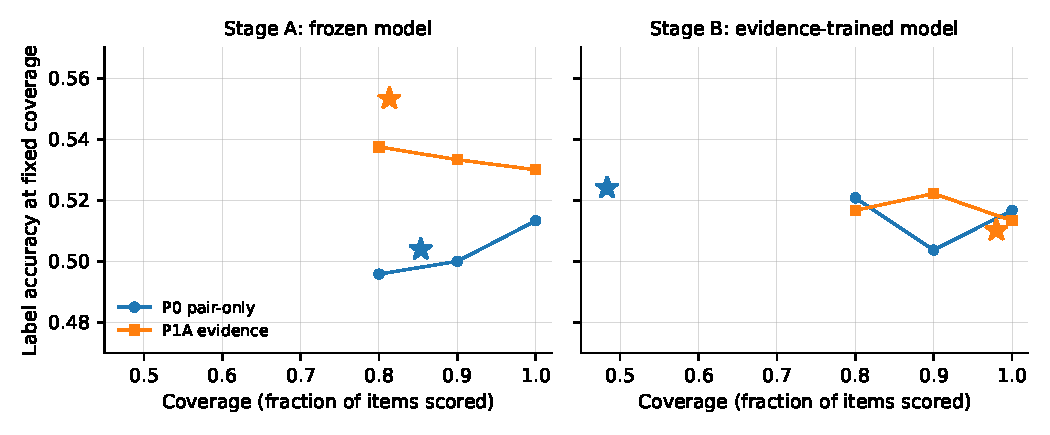
\includegraphics[width=\textwidth]{figures/fig_coverage.pdf}
\caption{Fixed-coverage accuracy for the probe's two stages (choice-confidence ranking; plain label accuracy on the most confident fraction, no arbitration). Stars mark accuracy among decided items, plotted at each arm's decided fraction. Stage A: the evidence arm is modestly ahead at every coverage level. Stage B: the arms sit within 0.014 of each other at every level, and pair-only is slightly ahead among decided items (0.5241 against 0.5102), while the headline accounting of Table~\ref{tab:stageb} separates them by 0.2467. The Stage B headline gap is produced by the decided fraction (0.9800 evidence against 0.4833 pair-only), not by accuracy where both arms commit.}
\label{fig:coverage}
\end{figure}

\subsection{Stage B: Evidence in Training, and the Pristine Collapse}
Stage B fine-tuned the base checkpoint on a 500-item train carve, each item in both question forms against its assembled evidence context (1,000 records; full arm, \texttt{soft\_ce}, vision tower frozen, 245 steps; loss 0.8468 to 0.7105). The carve is drawn from the training side and is disjoint from the validation-side probe items; within the carve, the train, tune, and calibration splits share no item and no image (670 unique images across its 700 items). Of the 500 items actually trained on, 74 had empty evidence blocks and trained with the question and no evidence text, kept deliberately so the tune split stayed representative. Under Amendment 6, the screen temperature and threshold were fitted on the reserved 100 calibration items only and frozen before the probe was scored: temperatures 0.0328 (pair-only) and 0.0300 (evidence), both near the fit floor because the tuned screen is near chance on calibration items (NLL 0.6929 at \(T=1\), 0.6897 fitted); thresholds 0.5456 and 0.5200.

\begin{table}[t]
\centering
\small
\caption{Stage B on the same 300 probe items (evidence-trained checkpoint).}
\label{tab:stageb}
\begin{tabular}{lccc}
\toprule
Arm & Headline acc & Acc incl.\ uncertain & Uncertain \\
\midrule
P0 pair-only & 0.2533 & 0.5167 & 155 \\
P1A evidence & 0.5000 & 0.5133 & 6 \\
P2A evidence & 0.5000 & 0.5133 & 6 \\
P1B evidence & 0.5067 & 0.5067 & 0 \\
\bottomrule
\end{tabular}
\end{table}

Headline accounting gives P1A a delta of \(+0.2467\), interval \([+0.2000, +0.2967]\). That number does not survive its own table. Accuracy including uncertain is flat (0.5133 against 0.5167). The pair-only arm abstains on 155 items and the evidence arm on 6; the decided fraction is 0.4833 against 0.9800, and among decided items pair-only is slightly ahead (0.5241 against 0.5102). At every fixed coverage level the arms sit within 0.014 of each other (Figure~\ref{fig:coverage}). The headline gap is produced entirely by the decided fraction: the Stage B headline is an abstention collapse, not an accuracy gain. This is the abstention-accounting standard at work: headline accuracy, accuracy including uncertain, decided fraction, and per-class headline recalls are co-primary here, and Table~\ref{tab:stagebclass} shows why the last of them is not optional.

\begin{table}[t]
\centering
\small
\caption{Stage B per-class reads (300 probe items; gold 152 pristine, 148 falsified). Choice recall scores the choice head alone; headline recall scores the arbitrated verdict.}
\label{tab:stagebclass}
\begin{tabular}{llcccc}
\toprule
Arm & Class & Pred.\ \(n\) & Choice recall & Headline recall \\
\midrule
P0 & pristine & 145 & 0.5000 & 0.5000 \\
P0 & falsified & 155 & 0.5338 & 0.0000 \\
P1A & pristine & 294 & 0.9868 & 0.9868 \\
P1A & falsified & 6 & 0.0270 & 0.0000 \\
P1B & pristine & 300 & 1.0000 & 1.0000 \\
P1B & falsified & 0 & 0.0000 & 0.0000 \\
\bottomrule
\end{tabular}
\end{table}

The diagnosis underneath is sharper. The Stage B evidence model's choice head labels 294 of 300 items pristine; of 148 gold-falsified items, only 4 are labeled falsified, and all 4 are then nulled by the arbitration, because no Stage B fake probability reaches its fitted threshold on any item (P1A range 0.4986 to 0.5031 against the 0.52 threshold). Falsified accuracy under headline accounting is exactly 0 of 148, in all three evidence strata. The 0.5000 headline is carried entirely by pristine items (150 of 152 labeled pristine and decided). P1B is the limiting case: it labels all 300 items pristine, and its including-uncertain accuracy is exactly the pristine base rate. The pair-only arm of the same checkpoint is the mirror failure: its choice head is near chance on both classes (Table~\ref{tab:stagebclass}), and the arbitration nulls all 79 of its correct falsified choices. Evidence training mostly taught the model to commit, and to commit to ``pristine''; where both arms commit, it is not more accurate. The Stage A winner shows the opposite default (it labels 273 of 300 items falsified). Any citation of the 0.5000 headline must carry the falsified-accuracy figure beside it.

Cross-stage, corrected: scored each under its own registered rule, Stage B P1A against Stage A P1A is \(+0.0500\), interval \([-0.0533, +0.1533]\), and Stage B P0 against Stage A P0 is \(-0.1767\), interval \([-0.2667, -0.0833]\). The pair-only sign reverses because the Stage B model abstains far more than the Stage A model under its own fit.

The carve's tune slice tells the same story at selection size. Judged on the 100 tune items through the audited path (Amendment 16), the Stage B checkpoint reads: P0 headline 0.21, including-uncertain 0.55, 63 uncertain; P1A headline 0.50, including-uncertain 0.50, 0 uncertain. The headline delta is \(+0.29\), interval \([0.20, 0.38]\), and it is entirely the abstention asymmetry: the evidence arm labels every tune item pristine (pristine headline accuracy 1.0, 50 of 50; falsified 0.0, 0 of 50), and including-uncertain the pair-only arm is ahead (0.55 against 0.50). No reading of the tune slice supports an evidence gain either.

\subsection{The Scorer Defect and the Audit}
\label{sec:scorer}
Two stored fields in the Stage B results were wrong, and finding out why took a full audit. The board review flagged the file as internally inconsistent: a cross-stage delta of \(+0.4367\) that the file's own headline accuracies (0.50 against 0.45) cannot produce, beside a falsified accuracy of 0.0 that looked like a label error. The audit recomputed every Stage A and Stage B figure from the canonical prediction files through one code path, thresholds passed explicitly. Every arm figure, stratum figure, within-stage delta, and interval in both files reproduced exactly, including the 0.0. The two contradictions had two different causes. The falsified 0.0 is not a scorer error; it is the pristine collapse, present in the predictions themselves. The cross-stage deltas are a scorer defect: the Stage B scorer kept its thresholds in a module-level dict that its main routine overwrote with Stage B's fitted thresholds, and its verdict function read that global, so Stage A prediction rows were rescored at 0.5456 and 0.52 instead of the registered 0.5. That collapsed Stage A P1A headline accuracy from 0.4500 to 0.0633, and the stored \(+0.4367\) is exactly 0.5000 minus 0.0633. Both stored cross-stage values reproduce exactly when the defective path is repeated, which confirms the diagnosis; the corrected values are the ones reported above. The audit also froze the canonical record: the \(n=300\) generation of the Stage A and Stage B artifacts is frozen with SHA-256 hashes in a manifest; an earlier \(n=298\) generation (Stage B delta \(+0.2483\), P0 headline 0.2517) circulated in chat and in a status note and is superseded wherever it differs.

One audit item was settled separately. Arms P1A and P2A are numerically identical in both stages, reproduced from the prediction files. The identity is by data, not a bug: P1A judged the fact-check-excluded evidence block and P2A the fact-check-included block, but the assembled evidence for the 300 probe items contains zero fact-check-domain passages in every one of the 193 non-empty sets, so no fact-check material ever survived retrieval into the probe evidence. The wiring was correct in every judge script; deterministic judging of the same input returned the same output. The honest consequence is that the fact-check-inclusion question is untested by this probe, not answered negatively.

\subsection{The VERITE Four-Arm Track}
A group-aware split of the local 1,001 rows (seed 20261122) froze a held-out 200 (65 true, 65 miscaptioned, 70 out-of-context). The adapted arm's step budget was selected on a train-side tune carve: 245 steps (tune accuracy 0.35) over 490 (0.31), the loser reported per the registration.

\begin{table}[t]
\centering
\small
\caption{VERITE four arms on the held-out 200.}
\label{tab:verite4}
\begin{tabular}{lccccc}
\toprule
Arm & Acc & Macro-F1 & True & Miscap. & OOC \\
\midrule
BASE & 0.285 & 0.2154 & 0.2462 & 0.0000 & 0.5857 \\
TRANSFER (v1 winner) & 0.320 & 0.2855 & 0.6615 & 0.2000 & 0.1143 \\
EVIDENCE (adapted \(+\) evidence) & 0.325 & 0.2497 & 0.3077 & 0.0000 & 0.6429 \\
ADAPTED (245 steps) & 0.330 & 0.3310 & 0.3538 & 0.3846 & 0.2571 \\
\bottomrule
\end{tabular}
\end{table}

ADAPTED minus TRANSFER is \(+0.010\), interval \([-0.080, +0.095]\): the registered success criterion (lower bound above zero) is \textbf{NOT MET}. EVIDENCE minus BASE is \(+0.040\), interval \([-0.005, +0.090]\). The adapted arm has the most balanced per-class profile and the best macro-F1, and the evidence arm recovers out-of-context items (0.6429) at the cost of never calling miscaptioned. The confusion matrices sharpen that: BASE and EVIDENCE never predict ``miscaptioned'' at all (0 of 200 predictions), TRANSFER defaults to ``true'' (142 of 200), and ADAPTED is the only arm that uses all three labels at volume. A prediction recorded in the registration put ADAPTED in the low-to-mid 0.40s; it landed at 0.330, and the miss is on the record. BASE in this table is the base checkpoint read on the held-out 200 only; it is not the v1 zero-shot baseline of Table~\ref{tab:verite}, which covers all 1,001 rows.

Because the held-out numbers carry a mandatory not-comparable warning against published full-set VERITE figures, the arms were also scored on the full local set (Amendment 14, registered before running). The held-out-200 subsets of the new full-set predictions reproduce the registered track exactly for every arm, so the full-set numbers are on the registered instrument. The adapted checkpoint had to be reconstructed for this scoring: the tensor pulled from the first probe pod was found truncated when checked against its own header, so the arm was retrained under its registered recipe before any full-set number was reported. The retraining receipt matches the original run's log to full float precision (final loss and tune metrics identical), and the retrained checkpoint's labels agree with the original run's stored held-out predictions on all 200 common items.

\begin{table}[t]
\centering
\small
\caption{VERITE arms on the full local set (1,001 rows), Amendment 14. ADAPTED's full-set read is inflated by construction: 801 of the 1,001 rows are its train and tune side; its clean read stays the held-out 0.330. EVIDENCE has no full-set number: frozen snapshots exist only for the 200 held-out items, and no fresh retrieval was run.}
\label{tab:veritefull}
\begin{tabular}{lccccc}
\toprule
Arm & Acc & Macro-F1 & True & Miscap. & OOC \\
\midrule
BASE & 0.3526 & 0.2865 & 0.4260 & 0.0089 & 0.6338 \\
TRANSFER (v1 winner) & 0.3586 & 0.2901 & 0.8136 & 0.1568 & 0.0954 \\
ADAPTED (245 steps) & 0.4725 & 0.4635 & 0.6420 & 0.4467 & 0.3231 \\
EVIDENCE (200 of 1,001) & 0.325 & 0.2497 & 0.3077 & 0.0000 & 0.6429 \\
\bottomrule
\end{tabular}
\end{table}

BASE and TRANSFER are zero-shot, so their full-set numbers are clean descriptives; protocol differences from published systems still apply, and the v1 H3 verdict is untouched by any of these reads. The full-set BASE and TRANSFER reads differ slightly from the v1 reads of the same checkpoints on the same rows (0.3526 against 0.3467; 0.3586 against 0.3506): the Amendment 14 judging ran in a later session than the v1 evaluation, and each verdict in this paper rests on its own run's reads.

\subsection{The Screen Beside the Verdict}
The probe also read the binary screen itself on the 300 probe items (Amendment 6's two-stage, two-arm read). Screen AUC barely moves between stages and arms: Stage A pair-only 0.5911, evidence 0.5819; Stage B pair-only 0.5917, evidence 0.5798. Raw ECE runs 0.0131 and 0.0542 (Stage A pair-only and evidence) and 0.0182 and 0.0425 (Stage B). Evidence, in training or in context, did not make the screen a better discriminator on NewsCLIPpings. That flatness is part of why the drill-down of Section~\ref{sec:noul} was run at all.

\subsection{Registered Follow-On: the NewsCLIPpings Scale Probe}
The scale probe (Amendment 15, registered before running) trains the pair-only NewsCLIPpings recipe at 10,040 train items (204 tune items held out; 20,080 training records in the two question forms) for 4,900 steps and reads the result on the same 300 probe items through the audited path. Its purpose is narrow: Part I's NewsCLIPpings arm trained on 2,001 items, and the probe tests whether a roughly fivefold increase in training items moves the pair-only read at all.

It does not move it in the direction the small-data reading would hope. The scale model's headline accuracy is 0.0467, against Stage A P0's 0.4300 on the same items: a paired delta of \(-0.3833\), interval \([-0.4433, -0.3267]\). Accuracy including uncertain is at chance and flat (0.5000 against 0.5133), and the headline collapse is again an abstention movement: the scale model is uncertain on 274 of 300 items, against 44 for the smaller model, because its choice answer and its binary screen disagree on those items. Its per-class headline reads are 0.0132 on pristine and 0.0811 on falsified, where the smaller model's falsified headline was 0.8716. The verdict is registered in the same form as the run: the NewsCLIPpings null is not a data-size artifact, and it hardens at this scale. More data at this recipe bought disagreement, not decisions.
%%%%%%%%% EVIDENCEGATE %%%%%%%%%%


\section{The Noul Drill-Down: Wording, Fitting, and Transfer}
\label{sec:noul}
%%%%%%%%% NOUL DRILL-DOWN %%%%%%%%%%
\subsection{Design: Eighteen Frozen Wordings}
On NewsCLIPpings in Part I, the trained model's screen AUC was 0.529 and its mean confidence 0.5002: the screen ranked items almost at random and sat near 0.5 on nearly everything, while the choice question carried the verdicts. Amendment 11 asked whether a better wording, a fitted temperature, or a combination of wordings could make the screen worth trusting. Six wordings per dataset were frozen in writing before any screen ran; none was added or edited after results. W0 is the control in all three packs: it asks whether the dataset would assign the item a falsified, distorted, miscaptioned, or out-of-context label rather than its original, pristine, or true label, and states plainly that this is a benchmark-label estimate, not an independent fact-check. W1 to W5 keep the same two answer options and change only the framing: direct probability (W1), truth-framed or original-context framings (W2, W3), an entity or decomposed checklist (W3 on NewsCLIPpings), a conservative wording written to lower the false-alarm rate (W4), and a pairing-first or claim-framed wording (W5). Two further design elements ride with the wordings. The B3 battery takes the top three wordings by selection AUC, fits a temperature to each, and averages their probabilities; it deploys unless the best admissible single beats its gain by more than two points. And the registered admissibility rule, as corrected by the Amendment 11 addendum: a wording is admissible only if it first gains on AUC over the control, its false-alarm rate is no worse than the control's, and its accuracy gain, read at \(T=1\) and threshold 0.5, is at least \(+3\) points. Screens ran on the base checkpoint, all six wordings in one call per item, option orders averaged in logit space, raw logits captured so every later analysis could be done without re-judging.

\subsection{The Three Tune Screens}
\textbf{NewsCLIPpings} (tune, \(n=100\)). The control is the best instrument in the set: W0 AUC 0.5816, raw accuracy 0.51 at raw alpha 0.94, and fitted accuracy 0.56 at fitted alpha 0.08 with no wording change at all. Every variant's AUC is below the control's (W1 0.4240, W2 0.3656, W3 0.3992, W4 0.3860, W5 0.4464), and several sit below chance. The screen implementation, comparing each variant's fitted read against the control's raw baseline, recorded W5 as the deployment (fitted accuracy 0.54, fitted gain \(+0.03\) under that comparison).

\textbf{VERITE} (tune, \(n=100\)). W3 (original context) is the only variant with an AUC gain over the control: AUC 0.5677 against W0's 0.5252, fitted accuracy 0.62, fitted alpha 0.5556 against the control's 0.7222. Its raw gain, read at \(T=1\) and threshold 0.5 under the registered definitions, is \(-0.15\). W1 (direct probability) is the worst variant here (raw delta \(-0.24\)), the reverse of its MMFakeBench behaviour. The implementation deployed single W3.

\textbf{MMFakeBench} (tune and calibration pooled, \(n=210\) items, 105 \(+\) 105; test closed). Here the control is the broken instrument: W0 AUC 0.4266, below chance, raw accuracy 0.5810 at alpha 0.8254. Every variant beats it. W1 (direct probability) is the best single: AUC 0.6735, fitted accuracy 0.6857, fitted gain \(+0.1048\), fitted alpha 0.6190. The battery \([1, 2, 4]\) reads AUC 0.6580, fitted accuracy 0.6762, fitted gain \(+0.0952\), alpha 0.4127, with member agreement 0.60; under the two-point preference rule the battery deployed, with W1 recorded as the best admissible single behind it. One caution recorded at the time and kept here: this screen reused the same tune and calibration items that Part I used for selection and calibration, a contamination question the confirmation screen of Section~\ref{sec:closing} was built to answer.

\subsection{Corrected-Rule Verdicts}
The board review found that the screen implementation had applied a fitted-versus-raw comparison where the registered rule reads gain at \(T=1\) and threshold 0.5 against the baseline, with an AUC-gain leg in front of it. The repairs recomputed all eighteen screens from the captured logits under the corrected rule, fitted-versus-fitted frontier included. The verdicts:

\begin{itemize}
    \item \textbf{NewsCLIPpings: W0 stands.} No variant and not the battery has an AUC gain over the control, so the admissible set is empty. The recorded W5 deployment is a protocol deviation, disclosed here and in the repairs file; the W5 and battery training runs and the Phase-3 battery evaluation below stand as an exploratory arm under the implementation's rule. The reframe costs no positive claim, because that arm's Phase-3 read was null.
    \item \textbf{VERITE: W0 stands.} W3 clears the AUC leg and the alpha leg under both readings, but its registered gain is \(-0.15\), failing the \(+3\)-point winner leg. The fitted-versus-fitted frontier supports W3 (fitted gain \(+0.03\), fitted alpha no worse), which is the reading the implementation used; the difference is the gain definition, and it is recorded rather than silently kept. Phase 3 then showed the choice does not transfer either way.
    \item \textbf{MMFakeBench: the battery \([1, 2, 4]\) stands.} Every variant clears the AUC leg with alpha no worse, but every single's registered gain is negative, so no single is admissible; the battery is admissible on its fitted form (\(+0.0952\), alpha 0.4127) and the preference rule cannot displace it. It is the one deployment that survives the corrected rule, with one fragility noted: at threshold 0.5 instead of its fitted 0.475, the battery's accuracy is 0.4476, below the baseline's raw 0.5810.
\end{itemize}

\subsection{Phase 2: A Small Training Test}
Each dataset's Phase-1 form was trained small (base checkpoint, winner recipe, 245 steps) and read on tune. NewsCLIPpings: the single W5 arm reaches choice accuracy 0.50 with screen AUC 0.4252; the battery arm (members 0, 1, 5) reaches choice accuracy 0.50, battery AUC 0.5392, accuracy 0.50 at alpha 0.28; the battery is the Phase-2 winner. VERITE: the single W3 arm reaches choice accuracy 0.42, fitted accuracy 0.60 at fitted alpha 0.5556; the battery arm (members 0, 2, 3) reaches choice accuracy 0.31, battery AUC 0.6115, accuracy 0.54 at alpha 0.3333; the single is the Phase-2 winner. MMFakeBench (read on the 105 tune items): the single W1 arm reaches choice accuracy 0.6571, macro-F1 0.6562, screen AUC 0.8215, screen alpha 0.5313; the battery arm (\([1, 2, 4]\)) reaches choice accuracy 0.6000, macro-F1 0.6103, screen AUC 0.7539, alpha 0.3750. The single is the Phase-2 winner, and it is the form Phase 3 then evaluated.

The MMFakeBench form lineage, stated once: the battery \([1, 2, 4]\) is the Phase-1 deployment, the one form that survives the corrected rule on the tune screen; the Phase-2 training test was then won by the single W1 form, on the numbers above; and Phase 3 evaluated the Phase-2 winner, the single. The three sections' different answers are a sequence, not a disagreement.

\subsection{Phase 3: The Reporting Evaluations}
One frozen-form evaluation per dataset, on items the selection never used for fitting the form itself.

\textbf{NewsCLIPpings} (battery \([0, 1, 5]\), the trained battery checkpoint, probe \(n=300\)): accuracy 0.55, alpha 0.3355, AUC 0.5698; gain over the baseline screen \(+0.0067\), interval \([-0.0767, +0.0900]\). A null. The threshold sweep shows why the frozen point is fragile: the battery's probabilities are so compressed that the whole threshold grid produces three outcomes, calling everything fake below the frozen threshold, reading 0.5500 at it, and collapsing to near the pristine base rate one step up.

\textbf{VERITE} (single W3, \(T=1.5458\), frozen threshold 0.625, held-out \(n=200\)): accuracy 0.55 at the frozen threshold, alpha 0.6462, AUC 0.4764, below chance on held-out items. At threshold 0.5 its accuracy is 0.675, which is exactly the fake base rate (135 of 200) at alpha 1.0: the form calls everything fake and is right at the base rate. No threshold on the grid gives both accuracy above the base rate and alpha below 0.5.

MMFakeBench Phase 3 is a closing experiment and is reported in Section~\ref{sec:closing}, where it belongs: it is the one Phase 3 that did not come back null.

\subsection{The Temperature Lesson}
The drill-down's most durable result is not about wording. Sixteen of the eighteen fitted temperatures sit at the 12.0 grid cap. The control's own fitted read on NewsCLIPpings gains \(+0.05\) over its raw baseline with no wording change at all: fitting moved the numbers more than the words did. Split-half refits then show that most fitted temperatures and thresholds do not hold across halves of their own selection sets. The NewsCLIPpings battery's W0 member swings from 0.0285 to the cap depending on which 50 items fit it, and the full fit used 0.0580; a member temperature that swings across the whole range is not a measured constant, it is a symptom of fitting three temperatures on 100 items. VERITE's Phase-3 temperature is the stable exception (split halves 1.3654 and 1.7985 around the full fit 1.5458), and even there the apply-half accuracy spreads from 0.48 to 0.64 at 50 items per half. Wording selection on 100-item tune slices did not produce a held-out gain on either dataset that ran a Phase 3 in this section.
%%%%%%%%% NOUL DRILL-DOWN %%%%%%%%%%

\section{Closing Experiments}
\label{sec:closing}
%%%%%%%%% CLOSING EXPERIMENTS %%%%%%%%%%
Three runs closed the study, each registered before it ran, each scored on its registered or audited path. The MMFakeBench test set stayed closed throughout.

\subsection{MMFakeBench Phase 3 (Validation Only)}
The Phase-2-winning form (single wording W1, trained from the base checkpoint, full arm, \texttt{soft\_ce}, vision frozen, 245 steps, 980 records) was frozen (W1, temperature 2.462, threshold 0.65) and judged once on the confirmation partition: 300 items of the MMFakeBench validation grouped split that were never used in any screen, training, or calibration. The construction that makes this true: the grouped split partitions the same 1,000-item validation set into a development partition (700 items) and a confirmation partition (300 items), group-aware and item-disjoint by construction; all Part I training, selection, and calibration, and all drill-down screens, sit inside the development partition. Choice accuracy 0.5667, macro-F1 0.5292. Per-class recalls: original 0.4333, textual distortion 0.8667, visual distortion 0.4000, mismatch 0.4556. Predictions spread across all four classes (75, 105, 33, 87): no degenerate collapse, unlike the NewsCLIPpings and VERITE Phase-3 arms. The screen read at the frozen temperature and threshold: AUC 0.8730, accuracy 0.7967, alpha 0.2556, ECE 0.0713. Its per-class AUCs against original are 0.9531 (textual distortion), 0.9707 (visual distortion), and 0.7707 (mismatch): the screen is weakest exactly where the choice head is weakest. One provenance note: recomputing the screen read from the stored prediction file gives AUC 0.8775 against the stored evaluation's 0.8730, and no stored artifact establishes the mechanism of the difference; the stored values, produced by the registered evaluation at run time and the lower of the two reads, are the canonical ones reported here. The striking part is the contrast: the base model's W0 screen on the same items sits at AUC 0.4308. The fine-tune, not the wording alone, carries the discrimination; the wording chose what the fine-tune would teach.

\subsection{G12: The Confirmation Screen}
Amendment 12 re-ran the frozen six MMFakeBench wordings plus the B3 construction on the same 300 untouched confirmation items, base checkpoint, one-call capture. Purpose: confirm or refute the tune screen on items that played no part in choosing anything. G12 was originally scored with the same screen scorer as the tune screen, whose admissibility is computed on the fitted view; the board review required the corrected-rule recomputation as well, and it was run from the stored capture logits (no re-judging) through the repairs code path. Both readings are reported here.

Under the fitted reading, W1 is again the best single: AUC 0.5744, fitted delta \(+0.0833\), fitted alpha 0.7556, with W3 also fitted-admissible (\(+0.0700\)). Under the corrected registered rule the verdict reverses. The AUC leg passes for every variant (W1 0.5744, W2 0.5650, W3 0.5685, W4 0.5594, W5 0.5657, all against the control's 0.4308), and the raw alpha leg passes for every variant (W1 0.2111 against the control's 0.8333). The gain leg, read at \(T=1\) and threshold 0.5, fails for every variant: W1's raw delta is \(-0.1533\), interval \([-0.2433, -0.0633]\) (raw accuracy 0.4133 against the baseline's 0.5667), and the other variants are further behind (W2 \(-0.1867\), W3 \(-0.2067\), W4 \(-0.1267\), W5 \(-0.2033\)). The admissible set under the registered rule is empty, so on the confirmation items W0 stands, a stronger verdict than on tune, where the battery stood and every single failed. What replicates across item sets is W1's ranking: the AUC advantage and the fitted-read standing. What does not replicate is a registered gain.

The tune screen's battery preference does not replicate either. B3 recomputed on this set takes members \([1, 3, 5]\), not \([1, 2, 4]\), and is not admissible even on the fitted view (delta \(-0.0167\); at threshold 0.5 its accuracy is 0.3533); the fitted screen's own deployment rule returns single W1 here, and the corrected rule returns the control. Member agreement on tune was 0.60, and the battery's membership and standing both change across item sets. The battery's instability is itself a finding, and it is why the MMFakeBench battery deployment of Section~\ref{sec:noul}, which stands on its tune record under the corrected rule, is reported with its confirmation failure beside it rather than as a settled deployment.

\subsection{Arm W: Stage B with a Frozen Wikipedia Corpus}
The Wikipedia arm replaces live web retrieval with a frozen corpus: the English Wikipedia abstracts dump as captured on 2024-04-20 (the standalone dump has been discontinued upstream; the Wayback capture of the canonical file is the newest obtainable copy, bit-identical to the archived capture, its SHA-256 hash on file in the corpus source record), indexed as a SQLite FTS5 table of 6,806,684 articles. A coverage test on the 30 pilot items, using the items' frozen query lists and an entity match rule, covered 29 of 30 (the miss is a garbled caption whose only entity is an obscure organisation with no matching article). Coverage is corpus reach, not verdict value, and the corpus predates the study by about two and a half years by construction.

Amendment 13 replicated Stage B with this arm: each item's frozen queries searched the index, hits pooled in query order, deduped by title, capped at five passages, formatted exactly as the live-web evidence blocks. Coverage in this form was 700 of 700 carve items and 300 of 300 probe items; that is coverage of retrieval, not of relevance, against the live arm's 64.3 percent headline coverage. Training mirrored Stage B (500 train items, both question forms, base checkpoint, full arm, \texttt{soft\_ce}, vision frozen, 245 steps, 1,000 records), and the loss fell much harder than the live-web run: 1.0463 to 0.1859, against 0.8468 to 0.7105. The calibration fit needed heavy softening (temperatures 5.02 and 5.02, at the fit grid's ceiling; thresholds 0.5849 pair-only and 0.2981 evidence), and the unmodified fitter crashed on this model's saturated probabilities, so the fit used the identical algorithm with a numerical clip guard, documented in the run notes. Scoring went through the audited verdict path with thresholds passed explicitly, per-arm falsified accuracy reported from the start.

Results on the 300 probe items, fitted accounting: pair-only headline 0.4933, including-uncertain 0.5233, 16 uncertain, decided fraction 0.9467, falsified accuracy 0.9122 (135 of 148). Evidence headline 0.4433, including-uncertain 0.5567, 63 uncertain, decided fraction 0.7900, falsified accuracy 0.5541 (82 of 148). Paired delta: \(-0.0500\), interval \([-0.1167, +0.0200]\). At plain 0.5 thresholds the same predictions read pair-only 0.4867, evidence 0.5133, delta \(+0.0267\), interval \([-0.0500, +0.1067]\), falsified accuracy 0.9189 and 0.5203. The two threshold views disagree in sign and both intervals cross zero: there is no reliable headline effect of Wikipedia evidence for the Wiki-trained model.

What is solid in Arm W is the mirror image of Stage B. This model's pair-only arm does not show the pristine collapse: falsified accuracy 0.9122 against the live-web Stage B model's 0.0, and a pair-only headline of 0.4933 against 0.2533, each under its own registered fit. The evidence arm's including-uncertain edge (0.5567 against 0.5233) is bought with far weaker falsified detection (0.52 to 0.55 across the two views) and more abstention. Stage B's artifact ran in one direction (commit to pristine, abstain on falsified); Arm W's runs in the other (detect falsified pair-only, lose it when evidence is added). Neither direction is an accuracy gain. Together they say the abstention accounting is not a reporting nicety in this study; it is where the effects live.
%%%%%%%%% CLOSING EXPERIMENTS %%%%%%%%%%


\section{Situations Faced}
\label{sec:situations}
%%%%%%%%% SITUATIONS FACED %%%%%%%%%%
Five incidents shaped this study's results or its record. Each is stated plainly: what happened, how it was caught, what changed.

\textbf{Retrieval suspension.} The first EvidenceGate retrieval ran up to about 23 concurrent query streams, tripped the search backend's unusual-traffic suspension, and, with the fallback engine blocked by the network egress proxy, received empty result lists in silence for most items (481 of 600 probe pools empty). It was caught by counting pool sizes in the snapshot files rather than trusting the pipeline's success returns. What changed: retrieval was re-run serially with a circuit breaker and per-pair disk checkpointing, after a first repair attempt lost 400 repaired pairs that existed only in memory; the failed snapshots were kept as the record of the failure, and every repaired record carries a repaired flag and timestamp. A side test of reverse image search failed for two independent structural reasons (the engine is unreachable from this network, and the probe images are archive-held with no public URL), so binding evidence in this study comes from the text channel only.

\textbf{Driver-wedged pod.} The first replacement pod for the v2 judging phase accepted setup, but its GPU was wedged at the driver level: the device tool saw the card while the framework's CUDA initialisation failed with error 999, and no in-pod fix exists for that state. An earlier pod in the same phase was deployed but never reachable over SSH and was terminated unused at \$1.20 of idle burn. What changed: the wedged pod was terminated (about \$0.14) and replaced, and every later deployment ran a health gate, device listing plus an actual CUDA tensor operation, before any setup work. Part I had its own infrastructure episodes of the same family: a parallel evaluation engine whose first attempt deadlocked when forked workers inherited CUDA state (fixed by moving all workers to a spawn start method, then proven equivalent to the serial engine on 120 shared items with zero label mismatches and zero probability difference before it was trusted), and a training-data subset bug that wrote image paths valid only from another directory, caught by a 7-million-line skip stream before any receipt was written.

\textbf{Scorer defect.} The Stage B scorer's cross-stage deltas were computed by rescoring Stage A predictions at Stage B's fitted thresholds, through a module-level threshold dict its own main routine had overwritten. The stored \(+0.4367\) was an artifact of that path. It was caught by the board review's insistence that the file contradicted itself, and proven by an audit that recomputed every figure from the prediction files and reproduced both the correct fields and, by repeating the defective path, the wrong ones. What changed: the corrected deltas replaced the stored ones in every downstream document, the canonical artifacts were frozen with hashes, and the closing experiments were scored only through the audited verdict path with thresholds passed explicitly.

\textbf{Abstention accounting.} The Stage B headline (\(+0.2467\)) and, in mirror image, the Arm W evidence read both turned out to be movements in the decided fraction rather than in accuracy. The trap is structural: an arbitration that counts disagreement as uncertain, scored by a headline that counts uncertain as wrong, rewards any change that makes a model commit, including committing to one class. It was caught by the board's finding and made quantitative by the audit's fixed-coverage rescoring, which showed the Stage B arms within 0.014 of each other at every coverage level. What changed: accuracy including uncertain and decided fraction became co-primary in every Stage B and Arm W table, and per-arm falsified accuracy is reported from the start in the closing runs, so the same trap cannot hide in a new headline.

\textbf{Selection-rule deviation.} The drill-down screen implemented a fitted-versus-raw comparison where the registered rule, as corrected by its own addendum, reads gains at \(T=1\) and threshold 0.5. The deviation changed one deployment outright (NewsCLIPpings W5, where the registered outcome was ``W0 stands'') and one deployment's basis (VERITE W3). It was caught by the board review comparing the implementation against the registration text. What changed: all eighteen screens were recomputed from the captured logits under the corrected rule, the deviation is disclosed in the repairs file and in Section~\ref{sec:noul}, the affected runs are reframed as an exploratory arm, and no positive claim rests on them. The habit this produced generalises: a selection rule is part of the registration, and an implementation that quietly substitutes a nearby rule has changed the experiment.

Two smaller catches belong in the same ledger. In Part I, the VERITE transfer evaluation first scored the base checkpoint twice over, once through a pack registry pointer and once through an evaluation helper that silently reused a populated output directory regardless of checkpoint; it was caught by a differ check (543 of 1,001 predictions differ once the winner is actually scored) and H3 was held open until the verified re-run. And the Part I calibration verdict survived its own transfer failure only because the held-out check was run at all: the registered measurement stands, the qualification stands beside it, and the shipped product uses \(T=1.0\).

\section{Threats to Validity and Warnings}
\label{sec:threats}
%%%%%%%%% THREATS AND WARNINGS %%%%%%%%%%
\subsection{Threats to Validity}
The study's selection slices are small: 105 tune items chose the Part I winner, 100-item tune slices ran the drill-down screens, and the probe reads rest on 300 items, so intervals around the Part II deltas are wide and several verdicts are ``not confirmed'' rather than ``refuted at size''. The MMFakeBench drill-down screen reused the tune and calibration items that Part I used for selection and calibration; the confirmation partition answers that contamination question for the screen's ranking claim, and its registered-gain verdict is the stricter one reported. VERITE is scored on a local extraction of 1,001 rows of the official 1,000-item dataset, and the four-arm track's held-out 200 is a carve under this study's protocol, not the published full-set protocol; the full-set scoring of Section~\ref{sec:evidencegate} narrows but does not close that gap, because the adapted arm's full-set read is inflated by construction. The study is a single-model audit: one checkpoint family, one training library. Two internal unknowns are carried openly: the identity of the library's \texttt{rlcd} objective against the published methods that share the name is unverified, so the objective comparison is claimed only for the library objective as implemented; and the LoRA rank-32 collapse mechanism is unverified. Retrieval coverage bounds every evidence claim: headline coverage was 64.3 percent on the probe and 44.5 percent on the VERITE held-out items, the strata gradient is descriptive rather than causal, and the fact-check-inclusion contrast (P1A against P2A) is untested because no fact-check material survived into the probe evidence. The two VERITE adapted checkpoints from the first probe pod were not pulled (transfer limits); their predictions, the scored artifacts, are on file, and the checkpoints are re-creatable from the logged configuration, as the full-set scoring demonstrated. Finally, one competitor figure used in the protocol table (0.5866) carries an unverified split; its ranking position is conditional, and no claim rests on it.

\subsection{Warnings for Benchmark Users}
This section is one of the study's two named methodological contributions, collected so it can be cited as a unit. Four warnings, each measured in this study:

\begin{itemize}
    \item \textbf{Metadata leakage ceiling.} A rule that reads only the two provenance fields \texttt{text\_source} and \texttt{image\_source} scores 0.9150 macro-F1 on the MMFakeBench tune split, and 0.9150 accuracy and 0.8510 macro-F1 on the official test split. Any MMFakeBench number reported without a metadata ban should be read against that ceiling. The audit is deliberately narrow: it does not test content-based source cues such as watermarks or text style, so the ceiling demonstrates that a shortcut exists; it does not quantify every shortcut signal in the benchmark.
    \item \textbf{Calibration transfer harm.} A temperature fitted on one distribution can severely harm calibration on another: the calibration-fitted \(T=8.4214\) moves held-out ECE from 0.1056 to 0.3955, while a distribution-matched split-half fit (\(T=1.65\)) improves it from 0.0994 to 0.021 (Figure~\ref{fig:cal1}). Fit on the deployment distribution, or ship \(T=1.0\).
    \item \textbf{Fitted operating points are fragile at small \(n\).} Sixteen of eighteen fitted screen temperatures hit the grid cap; split-half refits swing across the full range; a frozen threshold can sit one grid step wide, with accuracy collapsing one step either side. A screen fitted on 100 items needs its confirmation run designed in from the start.
    \item \textbf{Abstention can manufacture a headline.} Under any arbitration that scores disagreement as uncertain and any headline that scores uncertain as wrong, a change that merely makes a model commit will read as a gain. The abstention-accounting standard of Section~\ref{sec:evidencegate} (headline, including-uncertain, decided fraction, and per-class headline recalls, co-primary) is the defence; the Stage B \(+0.2467\) and its Arm W mirror are the worked examples. A related instrument warning: live retrieval is not reproducible at a one-day lag (mean Jaccard 0.2161), so retrieval experiments should be run against frozen, hashed snapshots, and the MMFakeBench literature itself is fragmented across at least six incompatible protocols, so cross-paper comparisons need protocol labels before they need error bars.
\end{itemize}
%%%%%%%%% THREATS AND WARNINGS %%%%%%%%%%

\section{Conclusion}
\label{sec:conclusion}
%%%%%%%%% CONCLUSION %%%%%%%%%%
We presented one study in two registered parts: a pre-registered fine-tuning study of LAYA-Vision, a 201M-parameter typed-decision model, under a frozen protocol across MMFakeBench, NewsCLIPpings, and VERITE, and the follow-on probe those results motivated, which tested retrieved evidence at inference and in training and screened the wording of the model's binary screen. The contribution is not a new architecture or training algorithm; it is a pre-registered, receipted, low-cost evaluation procedure that makes dataset conditionalities and benchmark shortcuts visible, and then audits its own instruments when they fail.

What the whole record supports can be stated compactly. Small-data fine-tuning works where falsity is stylistic: on the official MMFakeBench test the winner reaches 0.6020 macro-F1 against a 0.2037 baseline, second overall and first among trained systems on that protocol, from 490 training examples; H1 and H4 stand. The same recipe does not transfer to per-item factual pairing: H2 and H3 are clean negatives, and the v2 VERITE adapted arm adds only \(+0.010\) over transfer with its interval across zero. Adaptation gains in this study are dataset-conditional. Retrieved evidence does not rescue the factual benchmarks under strict accounting: at the frozen model the gain is small and unconfirmed (\(+0.0200\), interval across zero), in training it is an abstention collapse whose headline (\(+0.2467\)) inverts under the co-primary accountings, and in a frozen Wikipedia corpus both threshold views cross zero with opposite signs. One wording result is real and narrower than it first looked: the direct-probability screen's ranking replicates on untouched items, and a model trained on that single wording posts a screen AUC of 0.8730 where the base model's screen sits at 0.4308, while under the corrected registered rule no single wording is admissible on either item set. Calibration fitted on one distribution can harm another, and a matched fit repairs it; H5 stands as registered, with that qualification as part of the claim.

The claims that died are reported with the same prominence: the Stage B evidence headline, the cross-stage improvement story (a scorer defect), the drill-down deployments on NewsCLIPpings and VERITE, the MMFakeBench battery as a settled deployment, Wikipedia evidence as a headline improvement, the EvidenceGate trigger as a selective routing device at its registered threshold, and the expectation that in-benchmark adaptation would lift VERITE accuracy. Methodologically, the study contributes the two named items of Section~\ref{sec:intro}: an abstention-accounting standard for arbitrated verdicts, and a warnings section for benchmark users (a 0.9150 metadata leakage ceiling, calibration-transfer harm, fragile fitted operating points, and the abstention trap), together with a protocol audit that separates official-test results from retrieval, validation, and private re-split regimes, and a complete cost and deviations ledger. The result is a fully reproducible, low-cost pre-registered study with public checkpoints and a demo, reported without softening negative outcomes.

%%%%%%%%% REFERENCES %%%%%%%%%%
\bibliography{bibliography}
\bibliographystyle{iclr2025_conference}
%%%%%%%%% REFERENCES %%%%%%%%%%

%%%%%%%%% Appendix %%%%%%%%%%
\appendix
\section{Pre-registration, Hypotheses, Amendments, and Deviations}
\label{app:protocol}
The five pre-registered hypotheses and their binary verdicts are as follows.
\begin{itemize}
    \item \textbf{H1 (MMFakeBench gain):} MET on test. The winner improves test macro-F1 from 0.2037 to 0.6020; paired-resampling 95\% CI lower bound is \(+0.3853\), and no per-class recall drops.
    \item \textbf{H2 (NewsCLIPpings trained arm):} NOT MET. Trained accuracy 0.5104 is outside the \(0.55\)--\(0.65\) band and short of the registered \(+6.24\)-point bar over the zero-shot figure.
    \item \textbf{H3 (VERITE transfer):} NOT MET. Transfer accuracy 0.3506 is outside the \(0.38\)--\(0.48\) band.
    \item \textbf{H4 (recall floor):} MET. Minimum per-class tune recall of the winner is 0.6129.
    \item \textbf{H5 (calibration):} MET as registered, with the qualification in Section 4.5.
\end{itemize}

Design amendments are disclosed as follows. Amendment (b) keeps the vision tower frozen in both arms because the library's training loop cannot unfreeze it; the full arm therefore trains the language encoder plus decision head only. Amendment (c) adds a NewsCLIPpings training arm carved from its official train split, with its H2 criterion re-aimed at that arm. Amendment (d) adds the supplementary ablation tier after the registered core; its receipts are isolated and never feed selection, calibration, or test-once scoring.

The following deviations are recorded faithfully. (1) Frozen vision tower per amendment (b). (2) NewsCLIPpings evaluation by streaming, with no archived image storage for evaluation. (3) NewsCLIPpings trained arm and saved training-subset exception. (4) Notebook-only execution on the run machine's Jupyter kernel. (5) Supplementary ablation tier. (6) NewsCLIPpings selection metric uses the native question form only because the two question forms have flipped label indices. (7) Inert tag in the executed NewsCLIPpings training cell, which never passed the dataset parameter; results are unaffected. (8) Carve manifest erratum: the manifest label reads 2,000 train items while the files contain 2,001. (9) VERITE transfer defect with two layers: the pack registry initially pointed to the base checkpoint, and a checkpoint-blind output-directory reuse cache defeated the first fix; a clean re-run protocol corrected this. (10) Calibration qualification in Section 4.5. (11) PASS 2 stream engine change after 709 serial rows; the parallel engine was restarted from row 0 and an equivalence gate on 120 shared items found zero label mismatches and bitwise identical probabilities.

The full receipt bundle includes timestamped pre-registration, amendments, deviations, and per-configuration receipts. To preserve double-blind review, no public checkpoint, demo, or receipt URLs are disclosed in this submission; the artifact pointers are recorded in the receipt bundle and omitted here. The metadata leakage audit uses only \( \texttt{text\_source} \) and \( \texttt{image\_source} \), and scores 0.9150 macro-F1 on tune, and 0.9150 accuracy / 0.8510 macro-F1 on test.

Part II was registered in the probe design document and its thirteen amendments, each written before the run it governed: the EvidenceGate design and arm definitions, the frozen probe and carve constructions, the Amendment 6 screen attunement, the Amendment 11 drill-down and its corrected-rule addendum, the Amendment 12 confirmation screen, the Amendment 13 Wikipedia arm, the Amendment 14 full-set VERITE scoring, the Amendment 15 scale probe, and the Amendment 16 tune read. Its deviations are the five incidents of Section~\ref{sec:situations}: the retrieval suspension and its two-stage repair, the driver-wedged and unreachable pods, the scorer defect (corrected values replace the stored ones everywhere), the abstention-accounting adoption, and the selection-rule deviation (the affected deployments reframed as an exploratory arm; no positive claim rests on them). The fact-check-inclusion contrast is recorded as untested, not negative, for the reason given in Section~\ref{sec:evidencegate}.

\section{Supplementary Tables and Reproducibility Checklist}
\label{app:tables}
For reproducibility, Table~\ref{tab:ablation} summarizes the supplementary ablation tier. The binding labelling rules are: LoRA learning rate is \( \texttt{lr\_lora}=0.001\); head-only fine-tuning is never called a linear probe; VERITE is described as 1,001 local rows of the official 1,000-item dataset; baseline comparisons carry a wording footnote; rlcd claims are scoped to this library's two objectives and this recipe; the full arm is described as encoder-plus-head with the vision tower frozen. Artifact pointers for public checkpoints and the demo are omitted from this draft.

\begin{table}[t]
\centering
\small
\caption{Supplementary ablation tier on MMFakeBench tune split.}
\label{tab:ablation}
\begin{tabular}{lc}
\toprule
Configuration & Tune macro-F1 \\
\midrule
Second seed, winner recipe & 0.7320 \\
Encoder LR \(2\times10^{-5}\), 735 steps & 0.7178 \\
Encoder LR \(2\times10^{-5}\), 490 steps & 0.6871 \\
Encoder LR \(5\times10^{-6}\), 735 steps & 0.6438 \\
Encoder LR \(5\times10^{-6}\), 490 steps & 0.6217 \\
LoRA r8, 490 steps & 0.7037 \\
LoRA r8, 735 steps & 0.6362 \\
LoRA r32, 735 steps & 0.2244 \\
LoRA r32, 490 steps & 0.1168 \\
Head-only soft-ce, 490 steps & 0.4238 \\
Head-only soft-ce, 735 steps & 0.3098 \\
Head-only rlcd, 735 steps & 0.4899 \\
Head-only rlcd, 490 steps & 0.2590 \\
Data size 122, 490 steps & 0.1168 \\
Data size 245, 490 steps & 0.3670 \\
Data size 490, 490 steps & 0.6598 \\
\bottomrule
\end{tabular}
\end{table}

\section{Execution Evidence}
\label{app:evidence}
The study was executed as a single notebook run, and the notebook is the run record: anyone can check each stage's input, process, and output in the executed cells without further explanation. Figure~\ref{fig:collage} reproduces verbatim excerpts of that record, covering the frozen configuration, the environment and GPU check, the grid results, winner selection, the test-once guard, and the final hypothesis verdicts.

\begin{figure}[p]
\centering
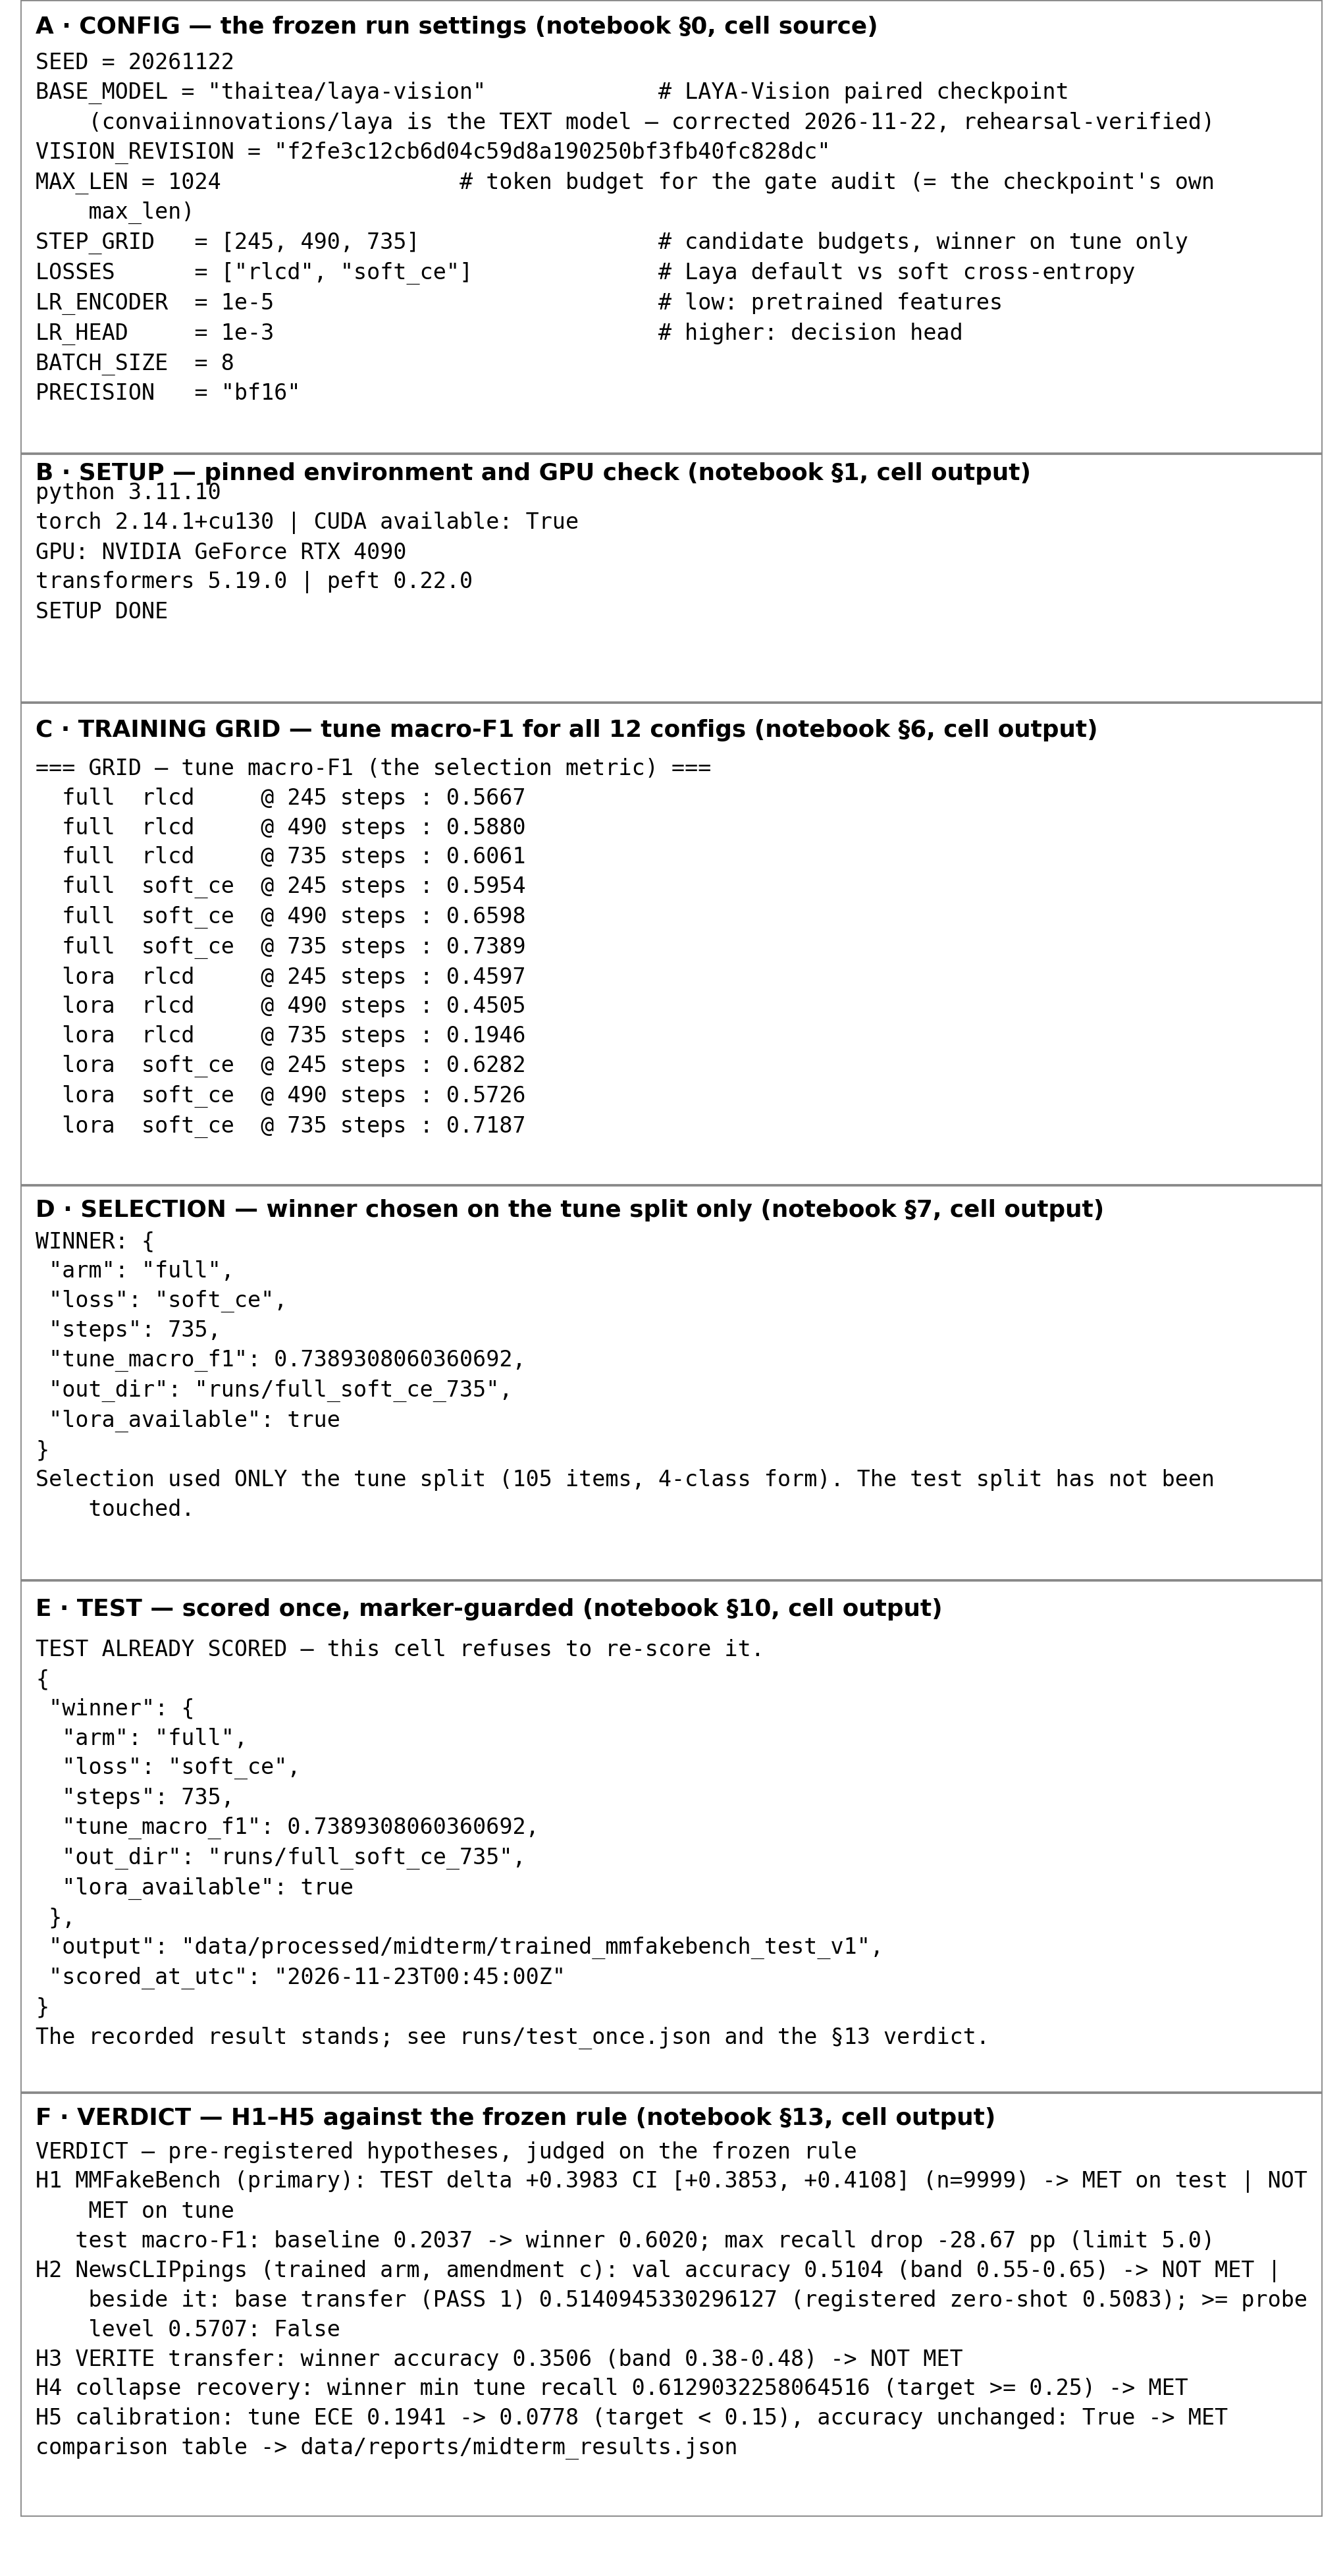
\includegraphics[width=\textwidth,height=0.89\textheight,keepaspectratio]{figures/collage_colab.png}
\caption{Execution evidence from the run notebook, reproduced verbatim. Panels show, in order: the frozen configuration; the pinned environment and GPU check; the training grid's tune macro-F1 table; winner selection on the tune split; the test-once marker, which refuses any re-scoring; and the H1--H5 verdicts computed against the frozen rule. Repeated library deprecation warnings are omitted from the excerpts; no values are altered.}
\label{fig:collage}
\end{figure}

\section{Code Appendix: Pseudocode}
\label{app:code}
This appendix compresses the study's own code into pseudocode. Each block is a faithful compression of the real code named in its subsection: the same steps in the same order, with the source's named constants, and no invented steps. The source files are versioned with this paper in the code folder of the study repository. Sections~\ref{app:code-verifier} and~\ref{app:code-parallel} describe components of Part I. Section~\ref{app:code-v2} documents the two probe components of Part II: the EvidenceGate state machine and the retrieval repair loop.

\subsection{The VisualNews Stream Verifier}
\label{app:code-verifier}
The verifier (\texttt{visualnews\_stream.py}) is the only route by which NewsCLIPpings evaluation images reach the model. The VisualNews archive is streamed once over HTTP and images are never written to disk. Member names in the archive are unreliable at source-dependent rates (payloads behind \texttt{.jpg} names are sometimes GIF, PNG, or BMP), so every decision is made on the decoded bytes, never on the extension. Only integrity failures skip; dataset properties (non-JPEG payloads, palette or RGBA modes, progressive JPEGs, animated images) never do.

{\footnotesize\begin{verbatim}
function verify_image_bytes(data):        # -> (ok, reason, image)
    if data is empty:
        return (False, "empty_member", None)
    try:
        img <- PIL open(data)      # format read from the bytes,
                                   # never from the member name
        if img.width * img.height > HARD_PIXEL_LIMIT:
            return (False, "oversize_dimensions", None)
                                   # 200,000,000 declared pixels:
                                   # refuse BEFORE allocating the
                                   # decode buffer
        img.load()                 # full decode, not a header
                                   # sniff: truncated payloads that
                                   # pass open() fail here. Animated
                                   # images decode frame 0, which is
                                   # what the pipeline judges.
    except any error e:
        return (False, reason_of(e), None)
                                   # "truncated" if the error
                                   # reports truncation, else
                                   # "decode_error"
    if img.width < MIN_DIMENSION or img.height < MIN_DIMENSION:
        return (False, "degenerate_dimensions", None)   # 8 pixels
    if img.mode is palette and it carries byte transparency:
        img <- img.convert("RGBA") # per PIL's own guidance, so
                                   # transparency is handled
    return (True, None, img.convert("RGB"))
\end{verbatim}}

{\footnotesize\begin{verbatim}
procedure stream_verified(source, referenced, on_image):
    wanted <- { normalize(p) : p  for p in referenced }
    ledger <- new SkipLedger
    ledger.note_referenced(each referenced path)
    stream <- open_stream(source)
      # a URL is fetched through a parallel range reader (range
      # segments served strictly in order; if the server does not
      # honour Range, fall back to a plain single stream); a local
      # path or an open file object is used directly. Socket reads
      # carry a 120 s inactivity timeout: a stalled stream raises.
    seen <- {}
    for member in tar_stream(stream, mode = "r|*"):
                                   # one pass, members consumed in
                                   # archive order
        if member is not a regular file: continue
        original <- wanted.get(normalize(member.name))
        if original is absent: continue
                                   # unreferenced: its payload is
                                   # never read; the stream reader
                                   # discards it as it advances
        seen.add(normalize(member.name))
        ledger.note_seen(original)
        data <- read member payload (empty bytes if none)
        (ok, reason, image) <- verify_image_bytes(data)
        if not ok:
            ledger.skip(original, reason); continue
        ledger.note_verified(original)
        results.append({ path: original,
                         prediction: on_image(original, image) })
    for each referenced path never seen in the stream:
        ledger.note_missing(path)
    return (results, ledger.summary())
    # summary(): referenced / seen / verified / skipped counts,
    # skip-reason counts, missing count, and the same accounting
    # per source (bbc, guardian, usa_today, washington_post,
    # other). A bad member never raises; only stream-level
    # failure raises, so the caller can restart the pass.

normalize(p): backslashes -> "/"; strip leading "./" segments
    and a leading "origin/" prefix. Applied identically to tar
    member names and to referenced paths before matching.
\end{verbatim}}

\subsection{The Parallel Stream Engine and Its Equivalence Gate}
\label{app:code-parallel}
The streamed validation pass of the NewsCLIPpings trained arm (PASS~2) was restarted on a parallel engine, because the serial pass is bounded by a single sequential tar traversal. The measurement procedure is identical to the serial engine's: same verifier semantics, same checkpoint, same pack questions, same temperatures, same prediction call, same row schema. Only execution concurrency changed, and the parallel engine was trusted only after the equivalence gate below passed. The worker processes live in \texttt{parallel\_stream\_engine.py}; the orchestration and the gate live in \texttt{parallel\_gate\_cell.py}, exported from the executed notebook cell.

{\footnotesize\begin{verbatim}
procedure run_parallel_pass(pack, checkpoint, rows, out_dir):
    groups <- rows grouped by image member (one image, many rows)
    saved  <- prediction rows already in out_dir (resume support)
    done   <- ids of saved rows with status ok
    start processes under the SPAWN context (never fork: CUDA
    cannot be re-initialised in a forked subprocess):
        1 reader process, 6 decode processes, 4 inference
        processes; queues byte_q (reader -> decoders), img_q
        (decoders -> inferers), evt_q (all -> coordinator)

    reader: stream the tar once, in archive order; for each
        member whose normalised name is wanted and not yet sent,
        emit a "seen" event and put (path, payload bytes) on
        byte_q; at end of stream signal reader_done (on stream
        failure, signal aborted instead)
    decoder (x6): loop on byte_q (stop on sentinel):
        verify_image_bytes(bytes); on failure emit skip(path,
        reason); on success emit verified(path) and put (path,
        image relayed as lossless PNG bytes) on img_q;
        then signal decode_done
    inferer (x4): load the checkpoint once; loop on img_q (stop
        on sentinel): for each row of this image whose id is not
        in done, predict with the pack's questions and
        temperatures and emit the item record on evt_q (status
        ok; blocked if the row's text is missing; error, with
        the exception counted, if predict raises);
        then signal infer_done
    coordinator (the single writer): consume evt_q; update the
        SkipLedger from seen / verified / skip events; append
        each item record to paired.predictions.jsonl, never
        writing an id already saved; when reader_done arrives,
        stop the decoders; when all decoders are done, stop the
        inferers; finish when all inferers report done
    dead-worker guard: if every inference process has exited
        without reporting done, abort loudly (the pipeline can
        never finish); likewise if all processes exit before
        their completion signals
    on abort: raise; scored rows stay on disk and resume
    reconciliation (only when not aborted): members skipped by
        the verifier or missing from the stream get explicit
        blocked rows for their unscored rows (reason recorded),
        so every referenced row is accounted for exactly once;
        metrics and per-source accounting follow from the
        completed prediction file

equivalence gate (runs before the full parallel pass):
    shared <- items scored by BOTH the preserved serial partial
              and a parallel run limited to the serial-scored
              members (serial file order is tar order, so the
              gate reads the tar head only)
    require |shared| >= 100
    require predicted labels identical on every shared item
    require max |p_parallel - p_serial| <= 0.001 on shared items
    any failure -> abort the restart; resume the serial pass
    executed run: 120 shared items, zero label mismatches, zero
    measured probability drift; the gate passed
\end{verbatim}}

\subsection{Part II Components: EvidenceGate and the Retrieval Repair}
\label{app:code-v2}
The two components below are the machinery of Part II (Sections~\ref{sec:evidencegate} to~\ref{sec:closing}): the EvidenceGate state machine that produced the probe's judgements, and the repair loop that repaired its retrieval instrument after the silent failure of Section~\ref{sec:situations}.

EvidenceGate is a pluggable per-item state machine around the paired judgement: it routes an item to a pair-only judgement or to a retrieve-then-judge path. Its configuration lives in the pack (\texttt{mode} in \{off, on, auto\}); with the gate off, behaviour is the Part I pipeline exactly. The specification is versioned in the probe design document.

{\footnotesize\begin{verbatim}
states:
    INTAKE    item + pack + checkpoint enter; the image is
              verified under the discipline of the verifier
              above
    ROUTE     the routing decision is computed and recorded,
              with its reason
    PAIR_ONLY the paired judgement of this study: pack questions
              verbatim, caption-only context. In mode auto its
              verdict is provisional.
    RETRIEVE  the retrieval pipeline below produces the item's
              frozen evidence bundle
    JUDGE     the model judges image + caption + evidence
              context with the registered evidence questions
    ARBITRATE the arbitration rule of this study: the choice
              verdict headlines; choice/noul disagreement gives
              verdict "uncertain"
    DONE      terminal: exactly one output record for the item
    ABSTAIN   terminal, unscored: integrity skip or
              unrecoverable model failure; counted in the run
              accounting. Distinct from "uncertain", which is a
              scored outcome produced by arbitration.

transitions and guards:
    INTAKE -> ROUTE        image verified; pack + gate load
    INTAKE -> ABSTAIN      verification fails (skip ledgered),
                           or pack/checkpoint cannot be loaded
    ROUTE -> PAIR_ONLY     mode off, or mode auto (pair first)
    ROUTE -> RETRIEVE      mode on
    PAIR_ONLY -> ARBITRATE mode off; or mode auto and the
                           trigger does not fire. Headline is
                           the pair-only verdict.
    PAIR_ONLY -> RETRIEVE  mode auto and the trigger fires; the
                           provisional pair-only verdict is kept
                           in the record as the control
    RETRIEVE -> JUDGE      bundle holds at least one passage
    RETRIEVE -> ARBITRATE  bundle empty or unusable; the
                           pair-only control verdict headlines
                           and the trace is flagged
    JUDGE -> ARBITRATE     always; headline is the evidence
                           verdict
    ARBITRATE -> DONE      always
    any -> ABSTAIN         predict raises, or a bundle's
                           snapshot hash check fails (never
                           judge on unverified evidence)

trigger (mode auto): the pair-only pass returns the choice
    distribution P and the noul fake probability q.
    margin       = largest P - second-largest P
    disagreement = (choice headline is fake-side) != (q >= 0.5)
    RETRIEVE fires iff margin < 0.20 or disagreement
    (both thresholds are registered knobs, frozen before any
    results; the trigger measurements are recorded in every
    item's state trace whether or not retrieval fires)

RETRIEVE, five steps (the search index is transport only: it
    fetches; it does not rank, select, or decide):
    1. extraction (deterministic): named entities plus noun
       chunks from the caption; variant A queries are built
       from these spans by a fixed template
    2. harness query expansion: a small model returns a
       one-line claim restating the caption and 2-3 further
       queries (variant B); it never sees gold labels or the
       image, and the claim text is used for queries only,
       never placed inside the judge's evidence block
    3. transport: both variants' queries issued to the search
       index (20 s per-query timeout); results unioned and
       deduplicated by URL; every result, used or not, is
       written into the snapshot with its URL, title, snippet,
       engine, timestamp, query, and variant
    4. triage: fact-check domains on the versioned
       contamination list and the item's own source article
       are excluded from the headline pools (kept in the
       snapshot, counted); results that merely repeat the
       caption's own claim are down-ranked, not deleted, and
       near-duplicate clusters collapse to their best member;
       survivors are ordered by whether they bear on the
       claim's checkable content (people, places, events,
       dates)
    5. selection + freeze: the top 5 passages, at most 600
       characters each, are selected in triage order and
       packed under the token budget; the bundle is written
       to disk and hashed (SHA-256); from this moment the
       item's evidence is fixed
\end{verbatim}}

The retrieval repair loop repaired a silent instrument failure in the probe's batch retrieval: concurrent query load tripped the search engine's suspension, and empty result lists were recorded as if they were results for most item-variants. The repair re-runs only the failed pairs, serially, with the items' frozen query lists and the same contamination rules.

{\footnotesize\begin{verbatim}
procedure repair_retrieval(items, raw_in, harness_in,
                           raw_out, harness_out):
    repair_list <- every (item, variant) whose recorded pool
                   size is 0
    new_raw <- all raw records except stale repair records for
               pairs in repair_list (untouched pairs are copied
               through verbatim; the original files remain as
               the pre-repair record)
    streak <- 0
    for each (item, variant) in repair_list:
        pool <- {}
        for q in the item's frozen query list (unchanged):
            results <- search(q)     # one query at a time; up
                                     # to 3 attempts, waiting
                                     # between attempts
            if results is empty:
                streak <- streak + 1
                if streak reaches 10:      # circuit breaker
                    sleep 240 s            # engine suspension:
                    streak <- 0            # pause, then resume
            else:
                streak <- 0
            for each result, in rank order:
                build its record (query, rank, URL, title,
                snippet, engine, score, published date,
                fact-check-domain flag, self-hit flag,
                timestamp, repair flag set)
                append the record to new_raw
                keep the best-scoring record per URL in pool
            sleep 1 s                # the disciplined rate
        record the item's new pool size for this variant
        try: re-run triage and passage selection on the pool;
             store the triage record and both passage sets
             (headline: fact-check excluded; second: included)
        on failure: store the error and empty passage sets,
             and count the failure
        mark the item repaired, with the repair timestamp
        flush both output files   # per-pair checkpoint: outputs
                                  # are rewritten atomically
                                  # after every pair, so a
                                  # stopped run loses nothing
    flush; write the run statistics (pairs repaired, harness
    calls and failures, balance before and after, spend)
    # pairs still empty after the repair are reported as
    # retrieval-failed, a different state from a genuine
    # no-evidence item, whose search ran and found nothing
\end{verbatim}}

%%%%%%%%% Appendix %%%%%%%%%%

\end{document}